\documentclass{article}
\usepackage{graphicx}
\usepackage{float}  
\usepackage[utf8]{inputenc}
\usepackage[includeheadfoot, margin=1em,headheight=2em]{geometry}
\usepackage{titling}
\usepackage{hyperref}
\geometry{a4paper, left=2cm, right=2cm, top=2cm, bottom=2cm}
\usepackage{graphicx}
\providecommand{\versionnumber}{1.0.0}
\usepackage{enumitem}
\usepackage[italian]{babel}
\usepackage{array}
\newcolumntype{P}[1]{>{\centering\arraybackslash}p{#1}}
\renewcommand{\arraystretch}{1.5} % Default value: 1
\setlength{\droptitle}{-6em}
\usepackage{capt-of}
\usepackage{setspace}
\usepackage{listings}

%font
\usepackage[defaultfam,tabular,lining]{montserrat}
\usepackage[T1]{fontenc}
\renewcommand*\oldstylenums[1]{{\fontfamily{Montserrat-TOsF}\selectfont #1}}

%custom bold 
\usepackage[outline]{contour}
\usepackage{xcolor}
\newcommand{\custombold}{\contour{black}}

%table colors
\usepackage{color, colortbl}
\definecolor{Blue}{rgb}{0.51,0.68,0.79}
\definecolor{LightBlue}{rgb}{0.82,0.87,0.90}
\definecolor{LighterBlue}{rgb}{0.93,0.95,0.96}

\usepackage{caption}
\captionsetup[figure]{labelformat=empty}

%Header
\usepackage{fancyhdr, xcolor}
\pagestyle{fancy}
\let\oldheadrule\headrule% Copy \headrule into \oldheadrule
\renewcommand{\headrule}{\color{Blue}\oldheadrule}% Add colour to \headrule
\renewcommand{\headrulewidth}{0.2em}
\fancyhead[L]{Manuale Utente}
\fancyhead[C]{Cybersorceres}
\fancyhead[R]{versione \versionnumber}

\title{\Huge{\textbf{Manuale Utente}}\vspace{-1em}}
\author{CyberSorcerers Team}
\date{}
\begin{document}
\maketitle
\vspace{-3em}
\begin{figure}[h]
  \centering
  
\includegraphics[width=6cm, height=6cm]{documenti/logo rotondo.png}
  \label{fig:immagine}
\end{figure}

\begin{center}
    \begin{tabular}{|l c c|}
    \hline
        \rowcolor{Blue} 
        \textbf{Informazioni sul documento} & &\\ [1 ex]
        \hline
        \rowcolor{LighterBlue}
        Destinatari: & Prof Tullio Vardanega & Prof Riccardo Cardin\\ [1 ex]
        \hline
    \end{tabular}
\end{center}


\vspace{6em}
\begin{center}
    \begin{tabular}{|P{24em}|}
    \hline
        \rowcolor{Blue}
        \textbf{Membri del team:}\\
        \hline
        \rowcolor{LighterBlue}
        \custombold{Sabrina Caniato}\\
        \hline
        \rowcolor{LightBlue}
        \custombold{Giulia Dentone}\\
        \hline
        \rowcolor{LighterBlue}
        \custombold{Nicola Lazzarin}\\
        \hline
        \rowcolor{LightBlue}
        \custombold{Giovanni Moretti}\\
        \hline
        \rowcolor{LighterBlue}
        \custombold{Andrea Rezzi}\\
        \hline
        \rowcolor{LightBlue}
        \custombold{Samuele Vignotto}\\
        \hline
    \end{tabular}
\end{center}

    
\newpage

\textbf{Registro dei Cambiamenti - Changelog\textsubscript{G}}
\begin{center}
\begin{tabular}{P{4em} P{6em} P{8em} P{8em} P{10em}}
  \rowcolor{Blue}
    \custombold{Versione} & \custombold{Data} & \custombold{Autore} &
    \custombold{ Verificatore} & \custombold{Dettaglio}\\
    \rowcolor{LighterBlue}
    1.0.0 & 26/05/2024 & Samuele Vignotto & Giovanni Moretti & Verifica finale del documento.\\
    \rowcolor{LightBlue}
    0.9.0 & 24/05/2024 & Sabrina Caniato & Giovanni Moretti & Aggiunta della sezione Istruzioni per il PlugIn.\\
    \rowcolor{LighterBlue}
    0.8.0 & 23/05/2024 & Nicola Lazzarin & Andrea Rezzi & Aggiunta della sezione Sviluppatore.\\
    \rowcolor{LightBlue}
    0.7.0 & 22/05/2024 & Giulia Dentone & Giovanni Moretti & Aggiunta della sezione Project Manager.\\
    \rowcolor{LighterBlue}
    0.6.0 & 21/05/2024 & Giulia Dentone & Sabrina Caniato & Aggiunta della sezione Cliente.\\
    \rowcolor{LighterBlue}
    0.5.0 & 21/05/2024 & Giovanni Moretti & Samuele Vignotto & Aggiunta della sezione Generale.\\
    \rowcolor{LightBlue}
    0.4.0 & 20/05/2024& Andrea Rezzi & Nicola Lazzarin & Aggiunta le istruzioni di login.\\
    \rowcolor{LighterBlue}
    0.3.0 & 13/05/2024 & Sabrina Caniato & Nicola Lazzarin & Aggiunta della sezione per l'installazione.\\
    \rowcolor{LightBlue}
    0.2.0 & 12/05/2024& Giulia Dentone & Sabrina Caniato & Aggiunta dei requisiti.\\
    \rowcolor{LighterBlue}
    0.1.1 & 05/05/2024 & Giulia Dentone & Samuele Vignotto & Aggiunta delle tabelle e compilazione della sezione di Supporto Tecnico.\\
    \rowcolor{LightBlue}
    0.0.1 & 03/05/2024 & Giulia Dentone & Samuele Vignotto &  Definizione struttura del documento e scheletro delle sezioni. Scrittura introduzione ed obiettivi delle diverse sezioni.\\
\end{tabular}
\end{center}
\newpage
\tableofcontents
\listoffigures
\listoftables
\newpage

\section{Introduzione}
\subsection{Scopo del documento}
Questo documento ha lo scopo di spiegare come utilizzare l'applicazione e illustrare le sue funzionalità. Fornisce informazioni sugli elementi essenziali necessari per far funzionare correttamente l'applicazione, spiega come installarla localmente e fornisce indicazioni su come utilizzarla in modo efficace.
\subsection{Scopo del prodotto}
L'azienda proponente ha richiesto la creazione di una web app che, tramite l'uso di IA (in questo caso ChatGPT4 e Bedrock) è in grado di creare epic user stories a partire dalle richieste del cliente e confrontarle con il codice sviluppato in modo da informare il cliente dello stato di avanzamento dello sviluppo del prodotto. Inoltre deve essere possibile, sia per il Project Manager, sia per il cliente rilasciare dei feedback (nel primo caso riguardanti l'adeguatezza delle stories, nel secondo caso riguardanti il prodotto finale) al fine di migliorare l'IA. È inoltre richiesta un' analisi comparativa tra le due IA utilizzate e lo sviluppo di un plug-in utile agli sviluppatori e al Project Manager.

\subsection{Glossario}
Alcuni termini presenti nel documento potrebbero essere ambigui, pertanto verranno inseriti nel Glossario v.1.0.0. La loro presenza all'interno di esso sarà indicata tramite una G maiuscola a pedice.

\section{Riferimenti}
\subsection{Riferimenti normativi}
\begin{itemize}
    \item Capitolato \textbf{C7 - ChatGPT vs BedRock developer Analysis}
    \\ \\
       \href{https://github.com/CyberSorceres/CyberSorceresRepository}{https://github.com/CyberSorceres/CyberSorceresRepository} 
    \item Norme del way of working v 1.0.0
    \item Regolamento del progetto didattico \\ \\ \href{https://www.math.unipd.it/~tullio/IS-1/2023/Dispense/PD2.pdf} 
    {https://www.math.unipd.it/~tullio/IS-1/2023/Dispense/PD2.pdf}
\end{itemize}
\subsection{Riferimenti informativi}
\begin{itemize}
    \item Slide del corso di Ingegneria del Software - Analisi dei requisiti \\ \\
    \href{https://www.math.unipd.it/~tullio/IS-1/2023/Dispense/T5.pdf}{https://www.math.unipd.it/~tullio/IS-1/2023/Dispense/T5.pdf}
    \item Slide del corso di Ingegneria del Software - Progettazione e programmazione: Diagrammi delle classi \\ \\
\href{https://www.math.unipd.it/~rcardin/swea/2023/Diagrammi%20delle%20Classi.pdf}{https://www.math.unipd.it/~rcardin/swea/2023/Diagrammi\%20delle\%20Classi.pdf}
\end{itemize}
\subsection{Riferimenti tecnici}
\begin{itemize}
\item Documentazione di React \\ \href{ https://react.dev/}{ https://react.dev/}
\item Documentazione di Typescript \\ \href{https://www.typescriptlang.org/docs/}{https://www.typescriptlang.org/docs/}
\item Documentazione di MongoDB \\ \href{https://www.mongodb.com/docs/}{https://www.mongodb.com/docs/}
\item Documentazione di Amazon AWS \\ \href{https://docs.aws.amazon.com/it_it/}{https://docs.aws.amazon.com/it\_it/}
\end{itemize}

\section{Requisiti}
Questa sezione fornisce un elenco dei requisiti minimi richiesti per eseguire l'applicazione, descrivendo le caratteristiche necessarie per configurare l'ambiente di sviluppo del progetto.
\subsection{Requisiti di sistema}
Affinché l'installazione e l'avvio del prodotto avvengano senza problemi e per garantire un'esperienza d'uso soddisfacente e completa dell'applicazione, è fondamentale installare i seguenti software.
\begin{center}
\begin{tabular}{|c|c|c|}
\hline
\rowcolor{Blue}
Componente & Versione & Riferimenti per il download \\
\hline
\rowcolor{LighterBlue}
Node.js & >=18.x.x & \href{https://nodejs.org/en/}{https://nodejs.org/en/}\\
\hline
\rowcolor{LightBlue}
npm & >=9.0.x & Integrato con il download di node.js\\
\hline
\end{tabular}
\end{center}
\captionof{table}{Tabella dei requisiti di sistema}
\label{tab:requisitist}

\subsection{Requisiti hardware}
Poiché l'applicazione viene eseguita tramite browser, non sono definiti requisiti specifici da parte del proponente, del capitolato o del progetto stesso. Di conseguenza, i seguenti requisiti sono indicati come linee guida generali per l'esecuzione del prodotto creato.
\begin{center}
\begin{tabular}{|c|c|}
\hline
\rowcolor{Blue}
Componente & Requisito \\
\hline
\rowcolor{LighterBlue}
Processore & Quad-Core 3,2 GHz\\
\hline
\rowcolor{LightBlue}
Memoria & 8GB DDR4\\
\hline
\rowcolor{LighterBlue}
Scheda grafica & Supporto a scheda grafica integrata con supporto OpenGL\\
\hline
\rowcolor{LightBlue}
Connessione internet & Connessione Internet stabile e veloce\\
\hline
\end{tabular}
\end{center}
\captionof{table}{Tabella dei requisiti hardware}
\label{tab:requisitihw}

\subsection{Requisiti software}
L'applicazione è stata testata sui browser più comuni, utilizzando le versioni iniziali come punto di partenza per lo sviluppo del progetto. Man mano che il progetto avanzava, sono state considerate progressivamente anche le versioni più recenti dei singoli browser.
\begin{center}
\begin{tabular}{|c|c|}
\hline
\rowcolor{Blue}
Browser & Versione \\
\hline
\rowcolor{LighterBlue}
Google Chrome & 110.0 \\
\hline
\rowcolor{LightBlue}
Mozilla Firefox & 109.0 \\
\hline
\rowcolor{LighterBlue}
Microsoft & Edge 110.0 \\
\hline
\rowcolor{LightBlue}
Safari & 16.0 \\
\hline
\rowcolor{LighterBlue}
Opera & 95.0 \\
\hline
\end{tabular}
\end{center}
\captionof{table}{Tabella dei requisiti software}
\label{tab:requisitisw} 

\vspace{1cm} Inoltre, come già menzionato, è necessario avere la versione 19.0 del software Node.js per poter utilizzare tutte le funzionalità del sistema e integrare senza problemi le ultime novità. Si raccomanda di utilizzare almeno la versione 17.0 per beneficiare completamente del supporto offerto dalla libreria.

\section{Installazione}
\subsection{Clonazione della repository}
Come prima cosa, per far funzionare la web app, è necessario che sia presente il codice nel pc che utilizzerà la web app. Esistono due alternative: 
\begin{enumerate}
    \item Scaricare il codice direttamente in formato .zip dal seguente link:\\
    \href{https://github.com/CyberSorceres/ProgettoFrontend}{https://github.com/CyberSorceres/ProgettoFrontend}
    \item Spostarsi nella cartella dove si vuole clonare la repository con il comando:
    \begin{lstlisting}
        cd path 
    \end{lstlisting}
    \item Clonare la repository da Git Hub con il seguente comando: \\
    \begin{lstlisting}
git clone https://github.com/CyberSorceres/ProgettoFrontend
    \end{lstlisting}
\end{enumerate}
\subsection{Avvio dell'applicazione}
Una volta clonata la repository, per poter avviare la web app servono un paio di passaggi:
\begin{enumerate}
    \item Aprire un terminale all'interno della cartella appena clonata.
    \item Al primo avvio usare il seguente comando per installare le dipendenza:
        \begin{lstlisting}
        npm ci
        \end{lstlisting}
    \item Fare la build con il comando:
        \begin{lstlisting}
        npm run dev
        \end{lstlisting}   
    \item Ora si aprirà una pagina sul browser predefinito al seguente indirizzo:\\\\
    \url{http://localhost:5173}
\end{enumerate}

\section{Istruzioni di utilizzo della web app}
\subsection{Login}
 \begin{figure}[H]
      \centering
      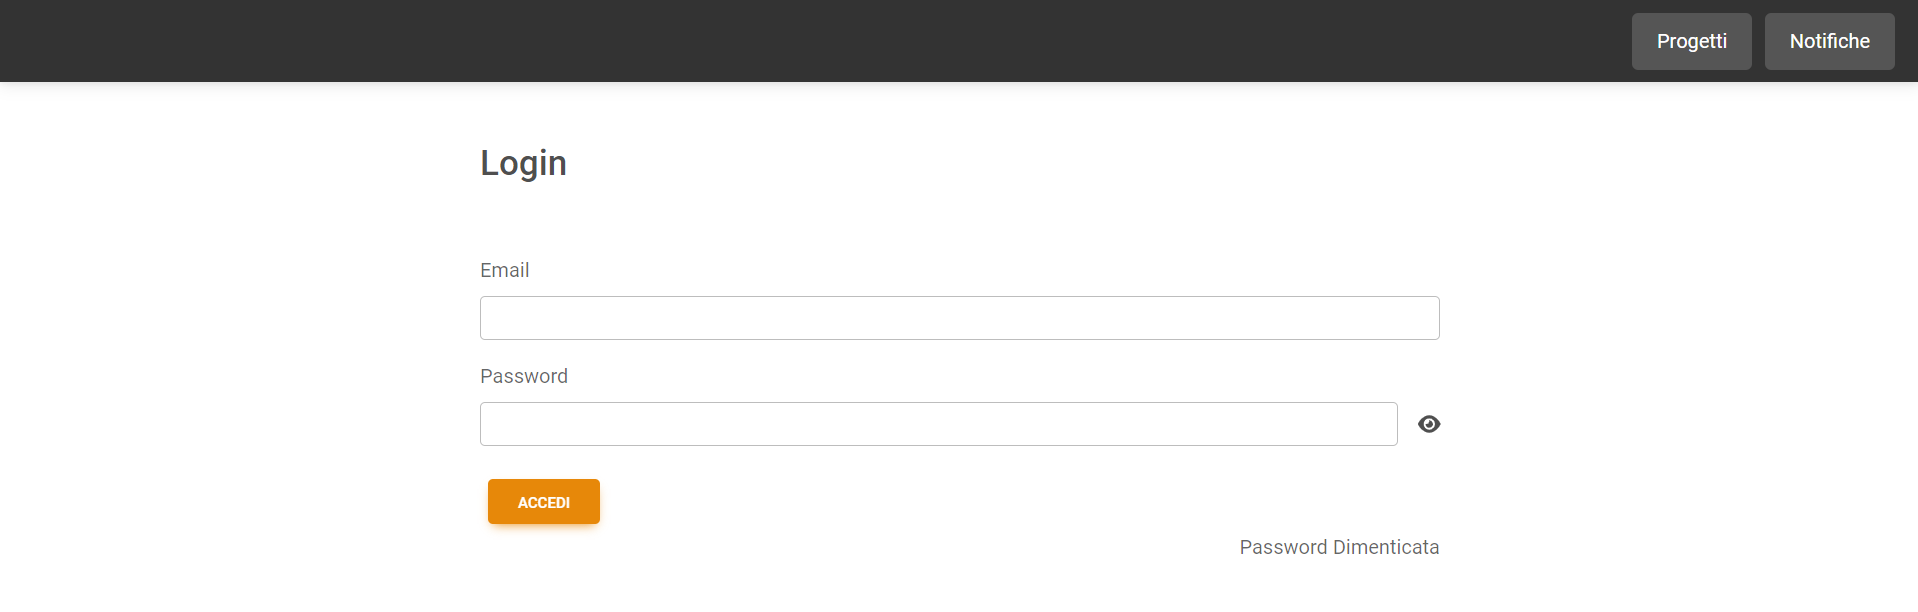
\includegraphics[width=\textwidth]{documenti/Screenshot manuale utente/pagina login.png}
      \captionof{figure}{Pagina di login}
      \label{login}
    \end{figure} 
Per effettuare il login all'interno dell'applicazione è necessario:
\begin{itemize}
    \item Inserire la propria email nel campo testo "Email";
    \item Inserire la propria password nel campo testo "Password";
    \item Cliccare sul tasto "Accedi".
\end{itemize}
La password durante l'inserimento non sarà visibile per ragioni di sicurezza, e apparirà nel seguente modo:
\begin{figure}[H]
      \centering
      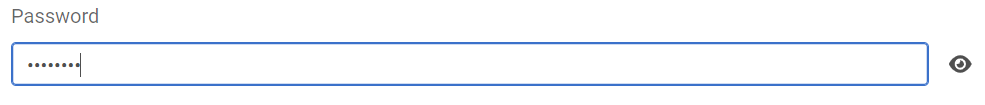
\includegraphics[width=\textwidth]{documenti/Screenshot manuale utente/password non visibile.png}
      \caption{Password nascosta}
      \label{passnascosta}
    \end{figure} 
Cliccando sull'icona dell'occhio a destra del campo testuale della password, quest'ultima diventerà visibile:
\begin{figure}[H]
      \centering
      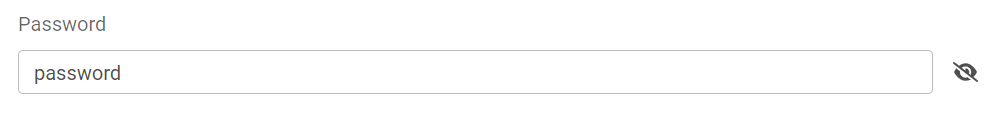
\includegraphics[width=\textwidth]{documenti/Screenshot manuale utente/password visibile.png}
      \caption{Password nascosta}
      \label{passvisibile}
    \end{figure}
Nel caso non si compilino i campi, che sono obbligatori, non sarà possibile effettuare il login e apparirà il seguente messaggio di avviso per invitare alla compilazione:
\begin{figure}[H]
      \centering
      
\includegraphics{documenti/Screenshot manuale utente/compila questo campo.png}
      \caption{Campi obbligatori non compilati}
      \label{campiobb}
    \end{figure}
Nel caso l'email inserita non sia presente nel sistema o la password inserita non sia corretta, apparirà il seguente messaggio di errore:
\begin{figure}[H]
      \centering
      
\includegraphics{documenti/Screenshot manuale utente/utente non esistente.jpeg}
      \caption{Utente o password errati}
      \label{errlog}
    \end{figure}


Nel caso si riscontrino problemi durante l'accesso provare a contattare il \hyperlink{linkSup}{supporto tecnico}. \\
Se lo username risulta inesistente contattare il \hyperlink{linkSup}{supporto tecnico}.

\subsection{Password dimenticata}
Nel caso la password venga dimenticata o si desideri modificarla, è possibile cliccare sul tasto "Passord dimenticata" presente in basso a destra, e comparirà il seguente modulo da compilare:
 \begin{figure}[H]
      \centering
      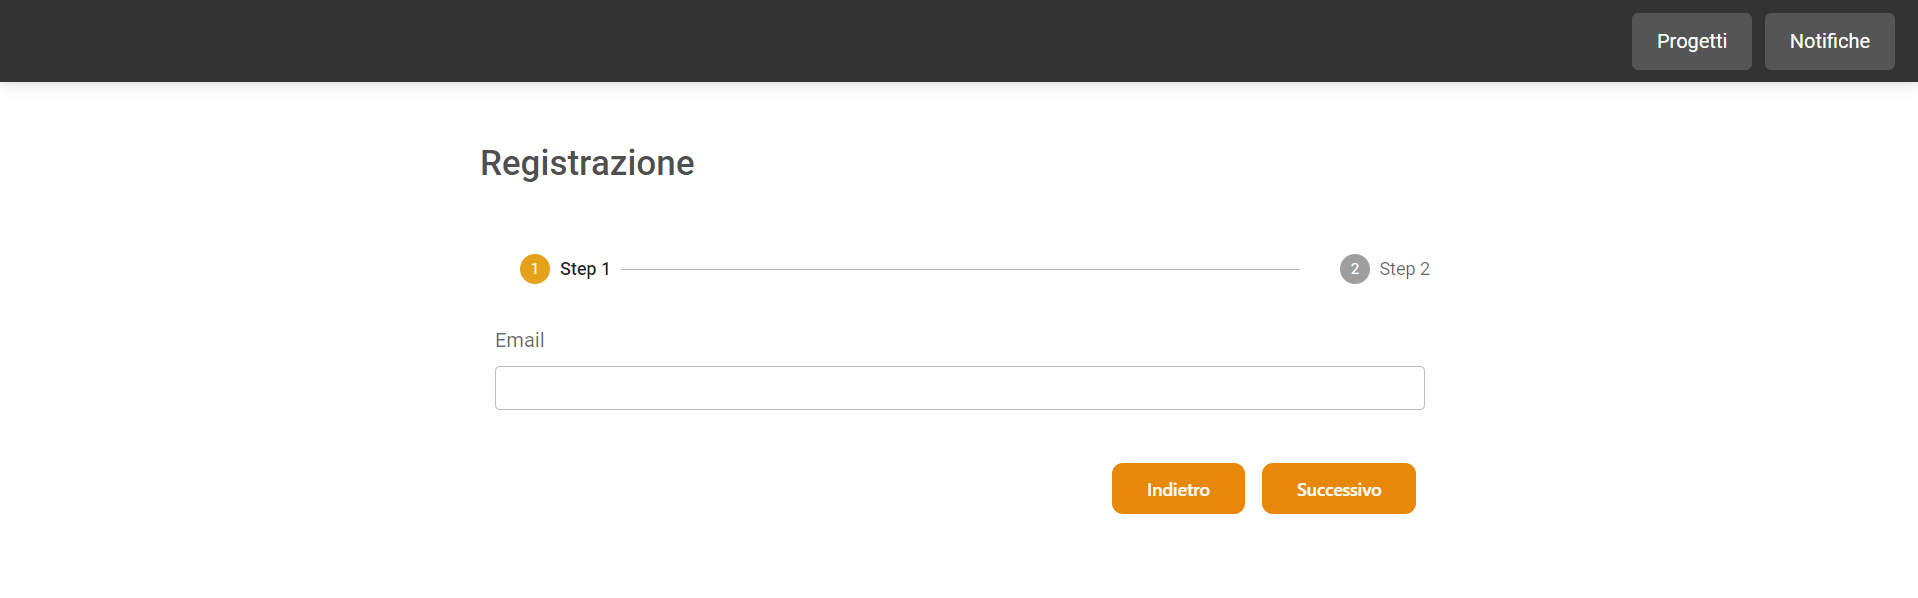
\includegraphics[width=\textwidth]{documenti/Screenshot manuale utente/cambio password step1.png}
      \caption{Password dimenticata o da modificare Step 1}
      \label{step1}
    \end{figure} 
ove bisogna:
\begin{itemize}
    \item Inserire la email nel campo testuale "Email";
    \item Cliccare il tasto "Successivo" per passare alla pagina successiva;
    \item Nel caso si desideri annullare l'operazione, è possibile cliccare il tasto "Indietro".
\end{itemize}
Nel caso si clicchi il pulsante "Successivo" senza aver compilato il campo "Email" obbligatorio, sarà visibile l'avviso:
\begin{figure}[H]
      \centering
      
\includegraphics{documenti/Screenshot manuale utente/compila questo campo.png}
      \caption{Campi obbligatori non compilati}
      \label{campiobb}
    \end{figure}
La pagina successiva si presenta nel seguente modo:
\begin{figure}[H]
      \centering
      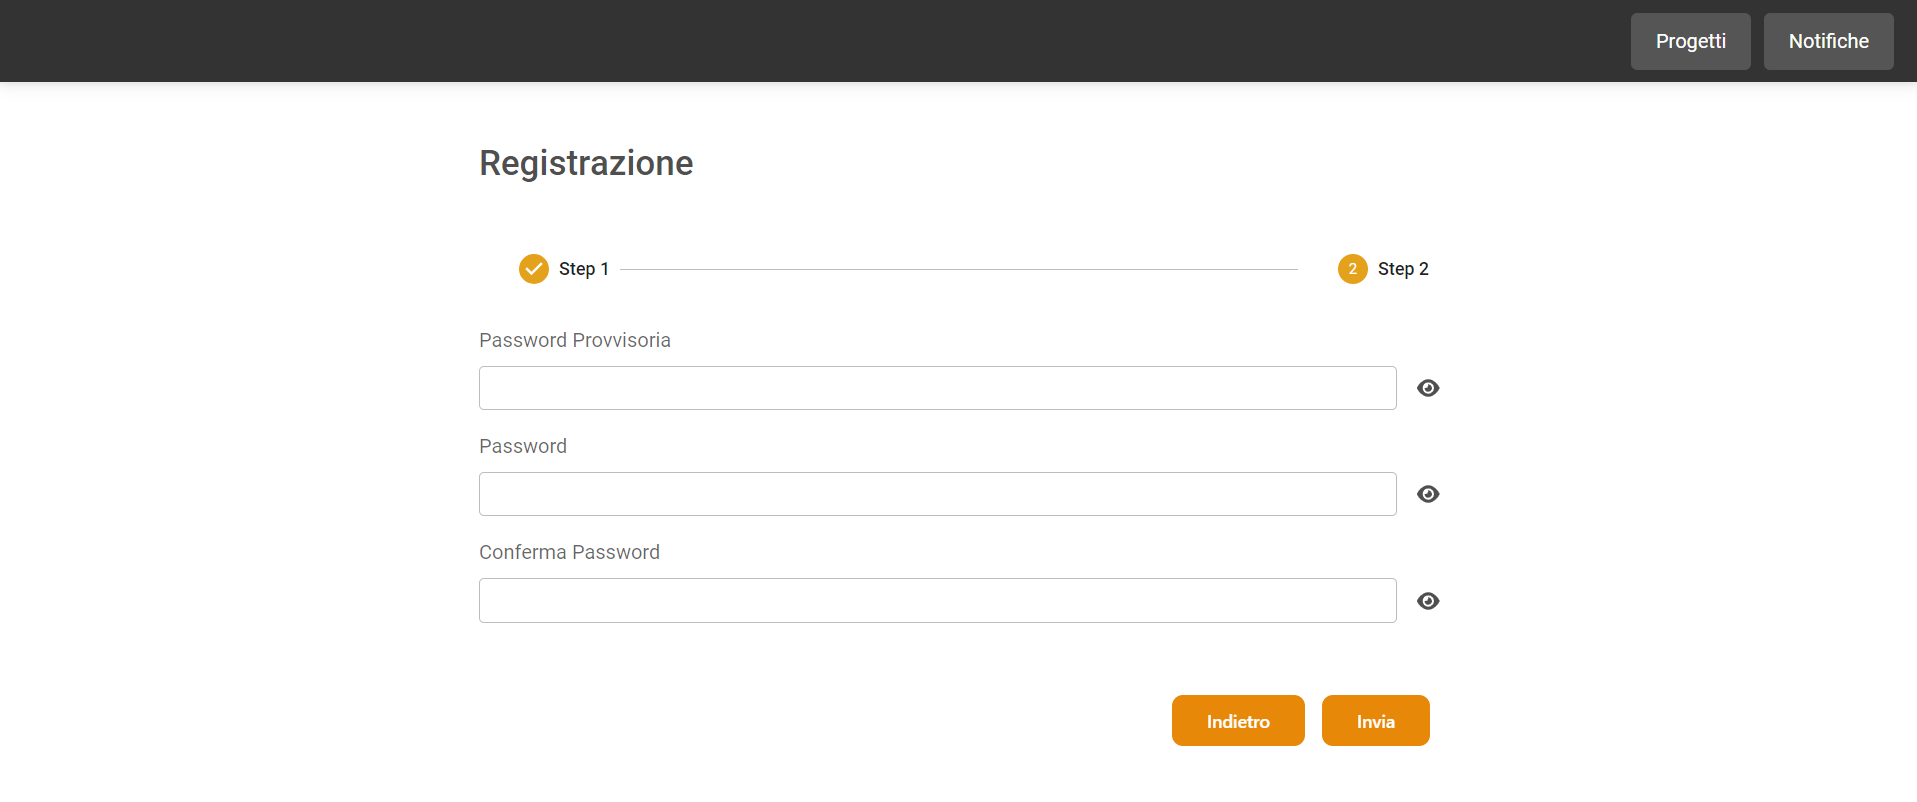
\includegraphics[width=\textwidth]{documenti/Screenshot manuale utente/cambio password step 2.png}
      \caption{Password dimenticata o da modificare Step 2}
      \label{step2}
    \end{figure} 
Per finalizzare l'operazione è necessario:
\begin{itemize}
    \item Inserire la password provvisoria arrivata via email nel campo testuale "Password provvisoria";
    \item Inserire la nuova password desiderata nel campo testuale "Password";
    \item Inserire la stessa password inserita nel campo "Password" nel campo testuale "Conferma password";
    \item Cliccare il tasto "Invia" per finalizzare la richiesta;
    \item Nel caso si desideri tornare allo Step uno è sufficiente cliccare il tasto "Indietro".
\end{itemize}
Nel caso si clicchi il pulsante "Successivo" senza aver compilato i campi "Password provvisoria", "Password" e "Conferma password" obbligatori, sarà visibile l'avviso:
\begin{figure}[H]
      \centering
      
\includegraphics{documenti/Screenshot manuale utente/compila questo campo.png}
      \caption{Campi obbligatori non compilati}
      \label{campiobb}
    \end{figure}
Nel caso le password inserite nei campi "Password" e "Conferma password" non corrispondano comparirà il seguente avviso:
\begin{figure}[H]
      \centering
      
\includegraphics{documenti/Screenshot manuale utente/password non corrispondono.png}
      \caption{Password non corrispondenti}
      \label{passdiverse}
    \end{figure}
L'avviso non indica quale dei due campi (email o password) sia errato per ragioni di sicurezza.

\subsection{Pagina inesistente}
Se l’utente cerca di accedere ad una pagina che non esiste, verrà reindirizzato alla seguente schermata, da cui in ogni momento potrà ritornare alla propria pagina principale;
\begin{figure}[H]
      \centering
      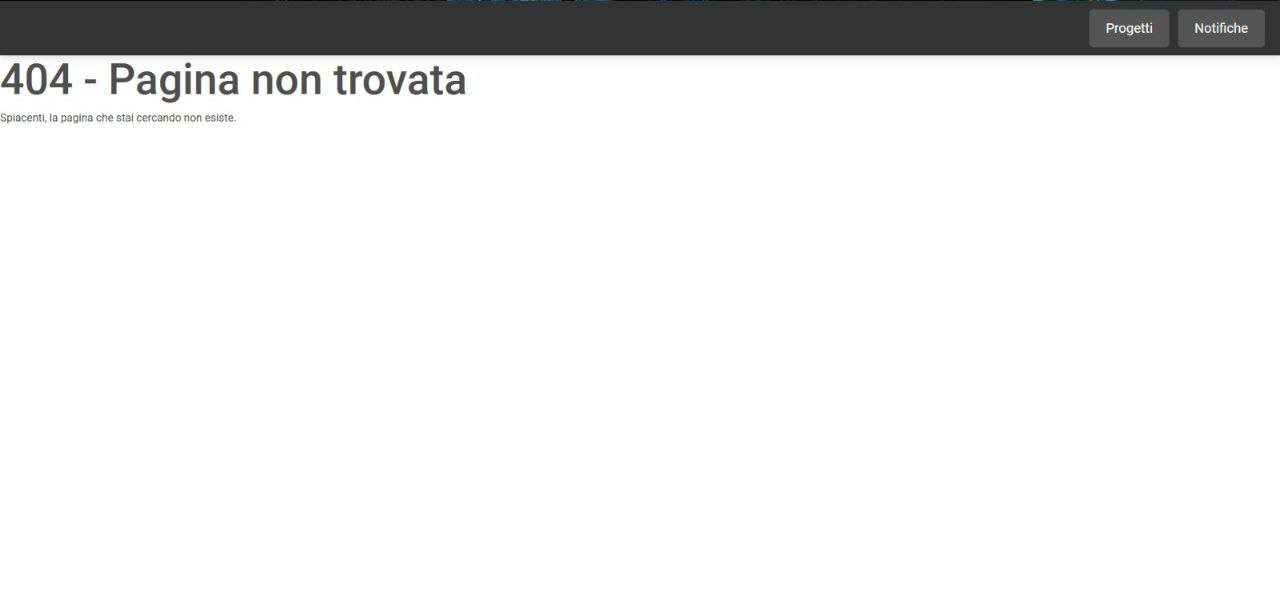
\includegraphics[width=\textwidth]{documenti/Screenshot manuale utente/pagina non trovata.jpeg}
      \caption{Pagina non trovata}
      \label{err404}
    \end{figure}
   
\section{Generale}
\subsection{Barra di navigazione}
 \begin{figure}[H]
      \centering
      
\includegraphics[width=\textwidth]{documenti/Screenshot manuale utente/navbar.png}
      \caption{Barra di navigazione}
      \label{navbar}
    \end{figure} 
La barra di navigazione è presente nella parte superiore della pagina e contiene: 
\begin{itemize}
    \item A sinistra il pulsante "Progetti" che, cliccato, riporta alla pagina dei Progetti a partire da qualsiasi pagina ci si trovi;
    \item A destra del pulsante "Progetti" è presente il pulsante "Notifiche", dove si possono visualizzare tutte le notifiche ricevute.
    \item A destra del pulsante "Notifiche" è presente il pulsante con una freccia per effettuare il logout dal proprio account. Una volta cliccato il logout si verrà automaticamente reindirizzati alla pagina di Login.
\end{itemize}

\subsection{Caricamento}
All'occorrenza di tutte le operazioni che richiederanno un caricamento e un'attesa da parte dell'utilizzatore verrà visualizzato il seguente messaggio di caricamento:
 \begin{figure}[H]
      \centering
      
\includegraphics{documenti/Screenshot manuale utente/caricamento in corso.png}
      \caption{Strumento di ricerca}
      \label{search}
    \end{figure} 
Non appena l'operazione sarà completata, il messaggio di caricamento scomparirà e verrà finalizzata l'operazione.

\subsection{Ricerca}
 \begin{figure}[H]
      \centering
      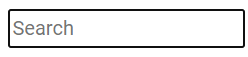
\includegraphics{documenti/Screenshot manuale utente/search.png}
      \caption{Caricamento in corso}
      \label{loading}
    \end{figure} 
Sarà possibile ricercare il progetto, l'Epic story o la User story desiderata all'interno delle tabelle scrivendo parole contenute nel loro nome all'interno del campo testuale. Lo strumento di ricerca sarà sempre posizionato in alto a destra all'interno della pagina. Una volta effettuata la ricerca, al posto di vedere tutti i componenti di una tabella, vedremo solo ciò che corrisponde al risultato della ricerca.

\subsection{Notifiche}
 \begin{figure}[H]
      \centering
      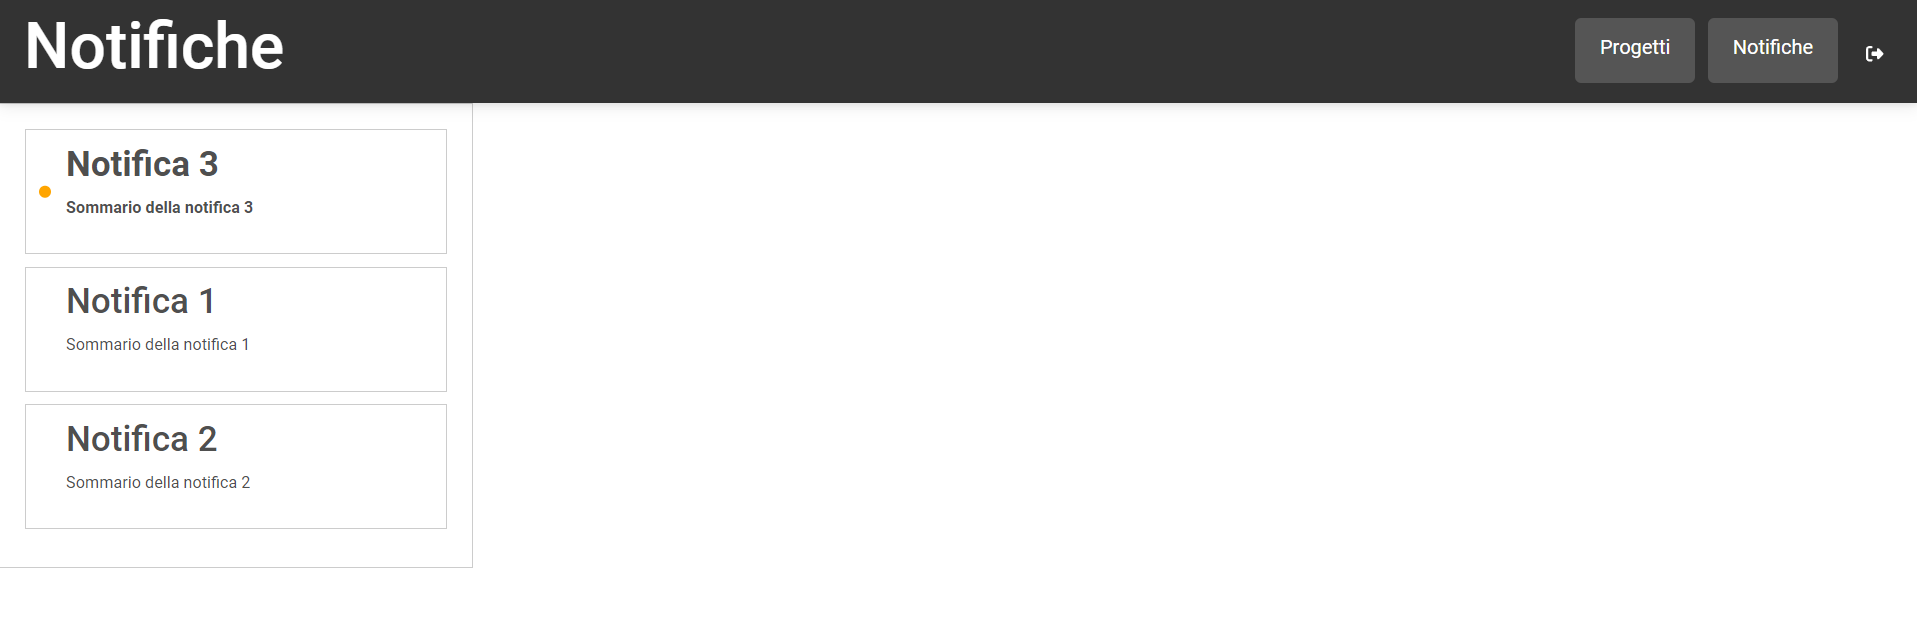
\includegraphics[width=\textwidth]{documenti/Screenshot manuale utente/notifiche.png}
      \caption{Pagina delle notifiche}
      \label{notifiche}
    \end{figure} 
In questa sezione si possono visionare le notifiche, che possono essere ricevute:
\begin{itemize}
    \item Se si è un Cliente, di un feedback ricevuto o il completamento di un progetto da parte dell'azienda.
    \item Se si è uno Sviluppatore, dell'assegnazione di una user story da parte del Project Manager;
    \item Se si è invitati da un Project Manager alla visione delle epic story di un progetto.
\end{itemize}
Cliccando su una delle notifiche sarà possibile visualizzarla nel dettaglio:
\begin{figure}[H]
      \centering
      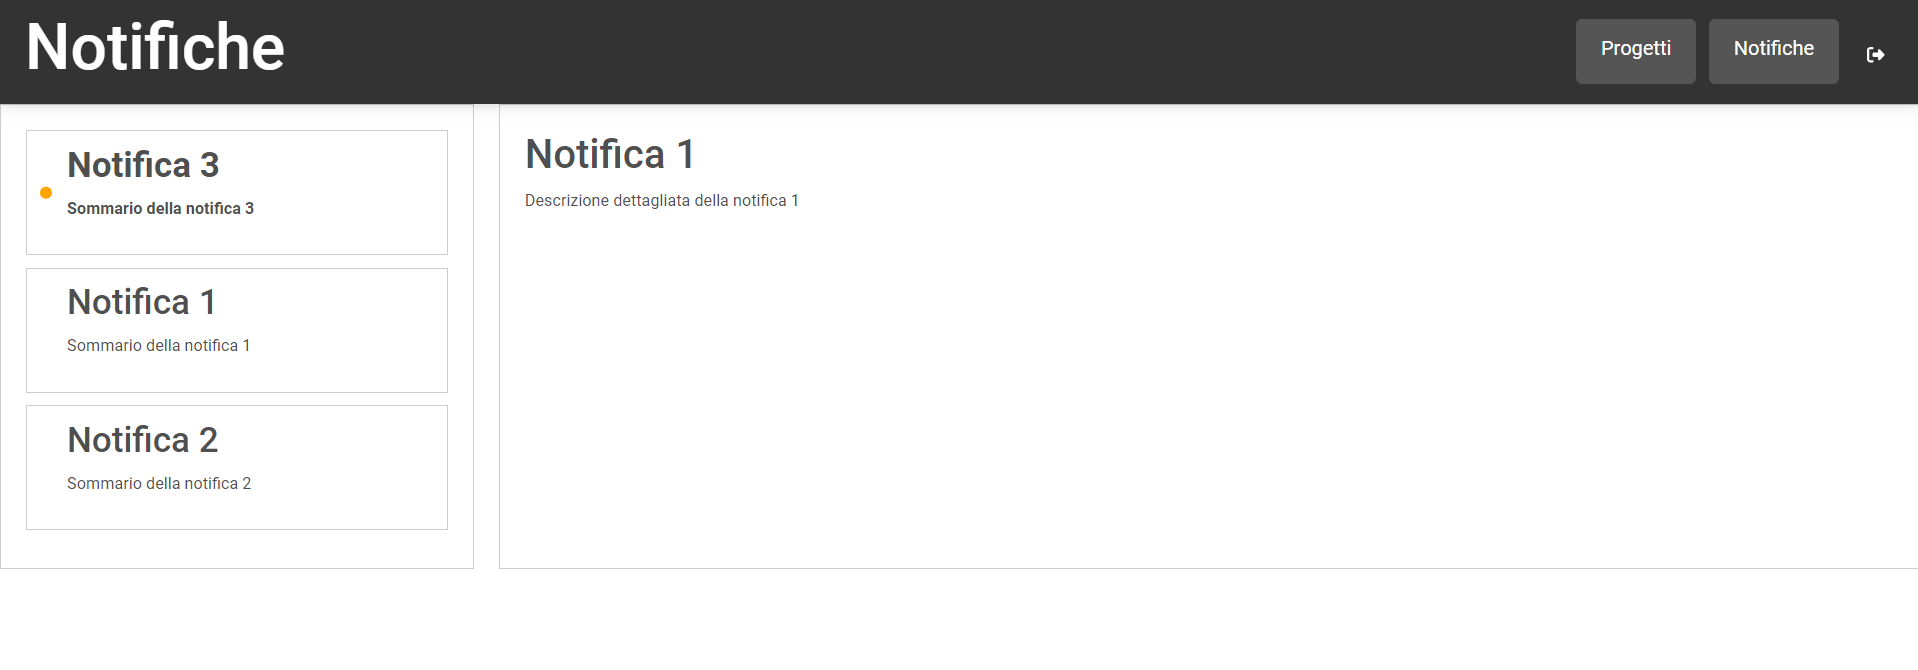
\includegraphics[width=\textwidth]{documenti/Screenshot manuale utente/dett not.png}
      \caption{Dettaglio della notifica}
      \label{notificadett}
    \end{figure} 
Sarà dunque visibile nel dettaglio la notifica. Cliccando su un'altra notifica verrà automaticamente sostituita quella presente sullo schermo con quella appena selezionata. Le notifiche non ancora lette, come mostrata la "Notifica 3", presenteranno il titolo in grassetto e un cerchio arancione a sinistra di esso. Non appena selezionate la prima volta, le notifiche saranno considerate lette e appariranno graficamente come le altre ("Notifica 1 e Notifica 2), e si sposteranno ai piedi della lista delle notifiche.\\
\\
Nel caso la notifica ricevuta sia un requisito di business, all'interno del dettaglio della notifica sarà presente il pulsante "Approva", sarà sufficiente cliccarlo per approvare la richiesta.
\begin{figure}[H]
      \centering
      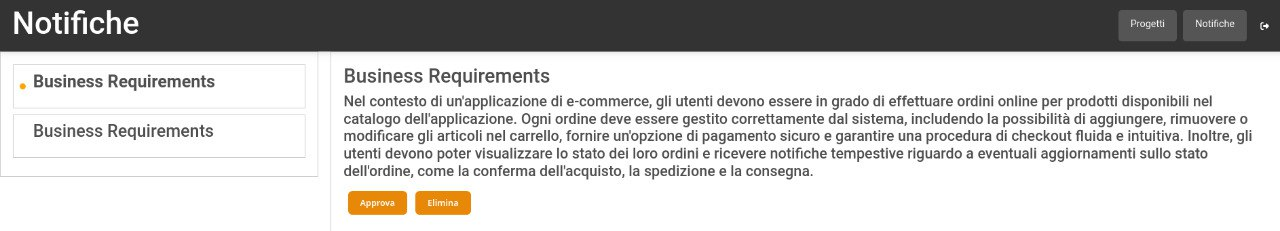
\includegraphics[width=\textwidth]{documenti/Screenshot manuale utente/notifica requisiti business.jpeg}
      \caption{Approvazione requisito di business}
      \label{notreqbusiness}
    \end{figure} 

\section{Cliente}
\subsection{Pagina dei progetti}
Questa è la pagina principale del Cliente:
 \begin{figure}[H]
      \centering
      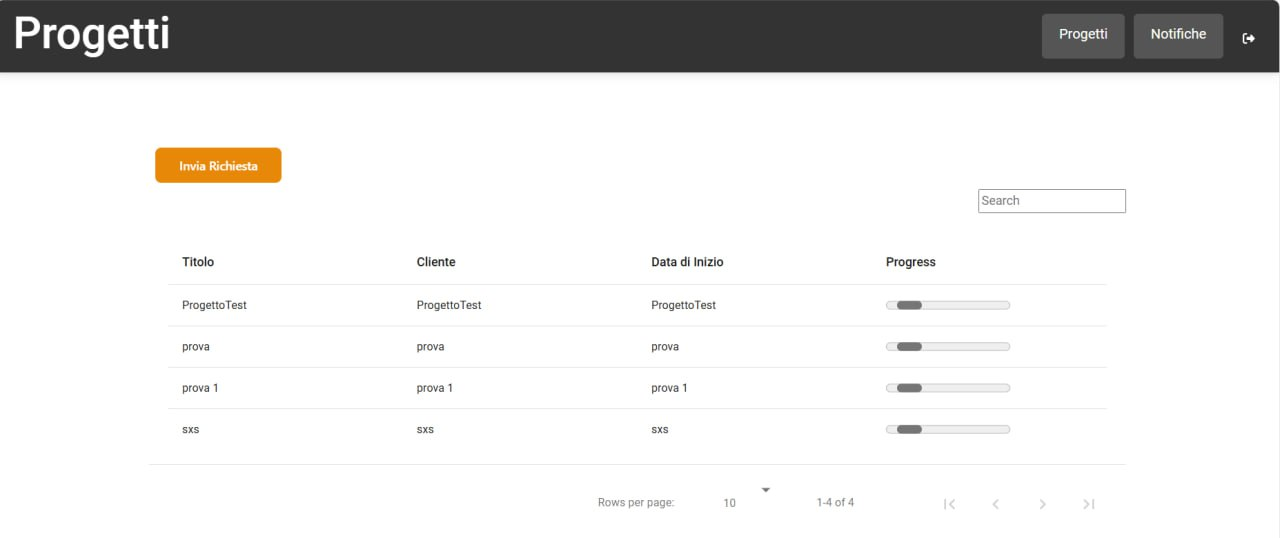
\includegraphics[width=\textwidth]{documenti/Screenshot manuale utente/home cliente.jpeg}
      \caption{Pagina principale del cliente}
      \label{pagcli}
    \end{figure} 
In questa pagina il Cliente può:
\begin{itemize}
    \item Visualizzare la lista dei progetti. Le colonne della tabella dei progetti sono:
    \begin{itemize}
        \item Il Titolo, che indica il titolo attribuito al progetto;
        \item Il Cliente, dunque chi ha commissionato il progetto;
        \item La Data di inizio, che indica la data di creazione del progetto;
        \item Il Progresso, cioè lo stato di avanzamento del progetto basato sulla percentuale di Epic e User stories completate.
    \end{itemize}
    \item Inviare richieste di business cliccando sul pulsante "Invia richiesta". Cliccando su questo pulsante apparirà il seguente pop-up:
     \begin{figure}[H]
    \centering
      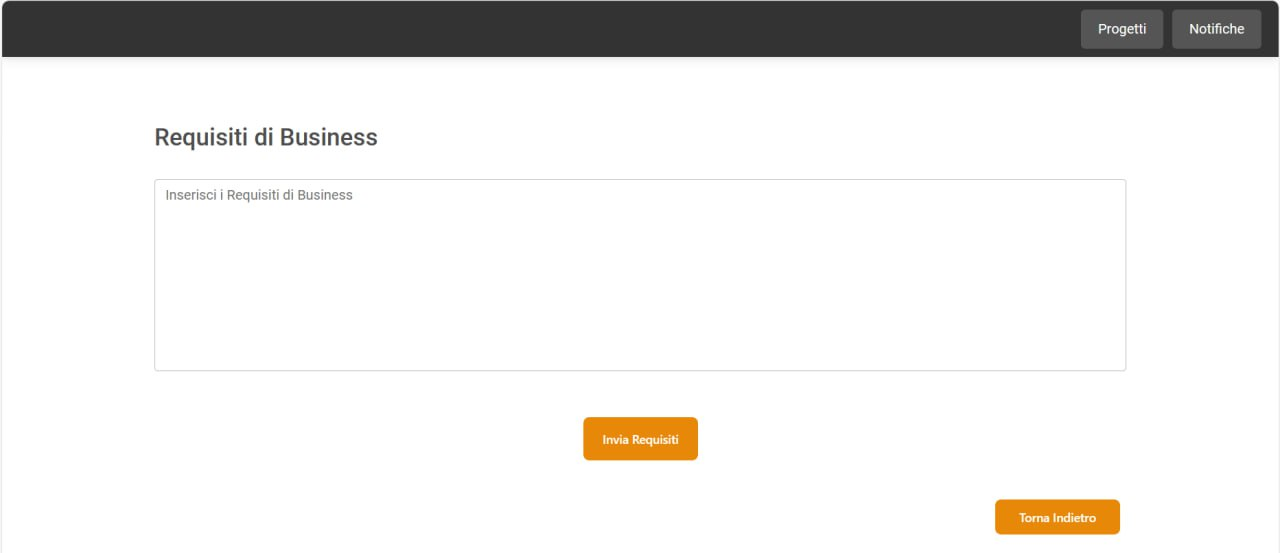
\includegraphics[width=\textwidth]{documenti/Screenshot manuale utente/invio requisiti cliente.jpeg}
      \caption{Invio di requisiti}
      \label{req}
    \end{figure} 
    Per inviare un requisito di business è necessario:
    \begin{itemize}
        \item Scrivere il requisito di business nel campo testuale;
        \item Cliccare il pulsante "Invia requisiti";
        \item Nel caso si desideri annullare l'operazione sarà sufficiente cliccare sul pulsante "Torna indietro" presente in basso a destra. 
    \end{itemize}
    \end{itemize}
    Cliccando sulla freccetta che compare andando sopra il titlolo di una colonna, è possibile invertire l'ordine alfabetico delle righe, A-Z oppure Z-A.
 è possibile inoltre andare alla pagina successiva nel caso i progetti siano troppo numerosi per essere visualizzati all'interno della pagina. 
    \begin{figure}[H]
      \centering
      
\includegraphics[width=\textwidth]{documenti/Screenshot manuale utente/cambio pagina.png}
      \caption{Cambio pagina della lista}
      \label{paginalista}
    \end{figure} 
    A sinistra sono indicate le righe per pagina, modificabili tramite il menù a tendina visionabile cliccando sulla freccia a sinistra del numero delle righe e scegliendo il numero desiderato:
        \begin{figure}[H]
      \centering
      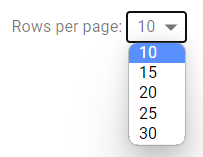
\includegraphics{documenti/Screenshot manuale utente/scelta righe per pagina.png}
      \caption{Scelta del numero di righe per pagina}
      \label{nrighepad}
    \end{figure} 
    è poi presente il numero della pagina in cui ci si trova rispetto al totale delle pagine, e le frecce per spostarsi all'interno di esse. Le frecce centrali permettono di spostarsi di una pagina rispettivamente precedente e successiva a quella in cui ci si trova, mentre le sue frecce esterne permettono di tornare rispettivamente alla prima o all'ultima pagina.


\subsubsection{Pagina delle Epic Stories}
Cliccando sulla riga del progetto di interesse (vedi immagine "Lista dei progetti), è possibile vedere le Epic story del relative a quel progetto:
    \begin{figure}[H]
      \centering
      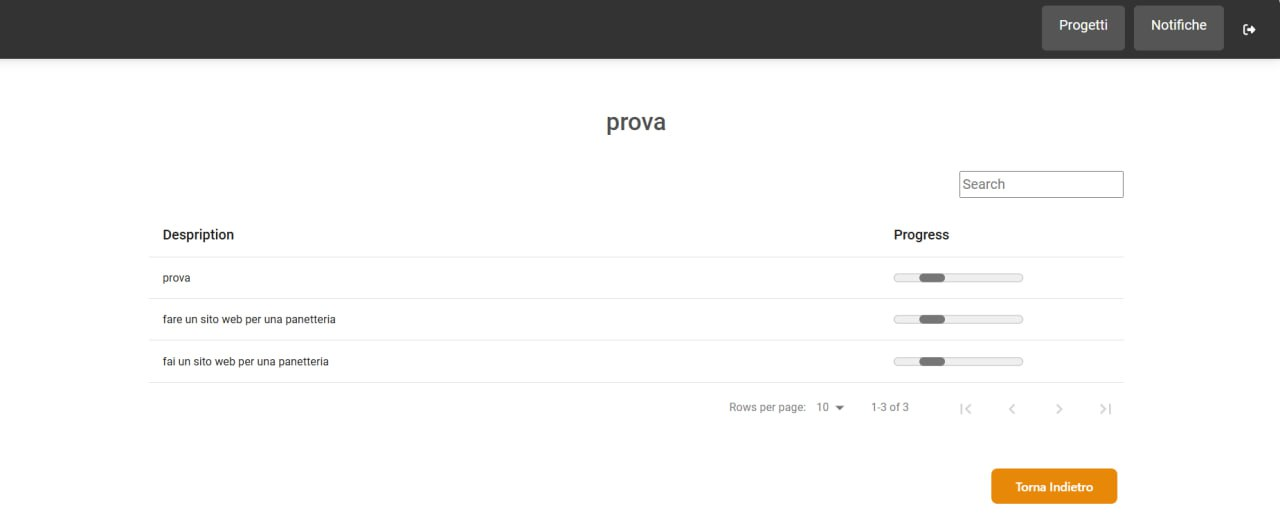
\includegraphics[width=\textwidth]{documenti/Screenshot manuale utente/epic dev.jpeg}
      \caption{Lista delle Epic stories}
      \label{listaepic}
    \end{figure} 
Le colonne della tabella indicano:
\begin{itemize}
    \item Il Nome delle Epic stories;
    \item Il Progress, ovvero una barra che indica lo stato di avanzamento delle Epic stories.
\end{itemize}
Cliccando sulla freccetta che compare andando sopra il titolo di una colonna, è possibile invertire l'ordine alfabetico delle righe, A-Z oppure Z-A.


\section{Project Manager}
\subsection{Pagina dei progetti}
Questa è la pagina principale del Project Manager:
 \begin{figure}[H]
      \centering
      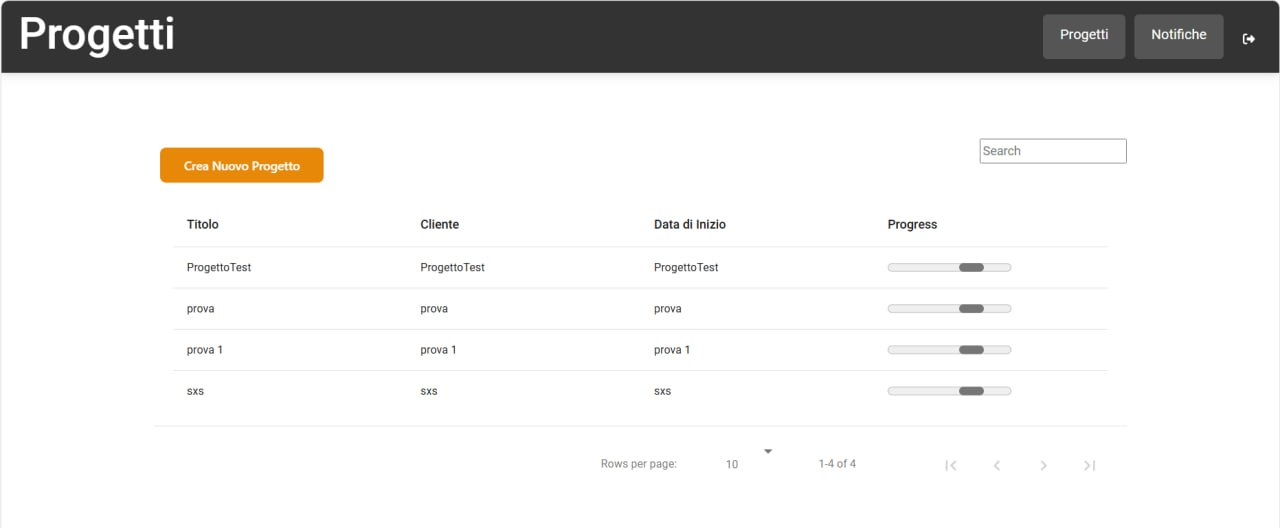
\includegraphics[width=\textwidth]{documenti/Screenshot manuale utente/progetti def.jpeg}
      \caption{Pagina principale del Project Manager}
      \label{pagpm}
    \end{figure} 
In questa pagina il Project Manager può:
\begin{itemize}
    \item Creare un progetto tramite il pulsante "Crea nuovo progetto"
    Una volta cliccato il pulsante "Crea nuovo progetto" apparirà un pop-up che si presenta nel seguente modo:
\begin{figure}[H]
      \centering
      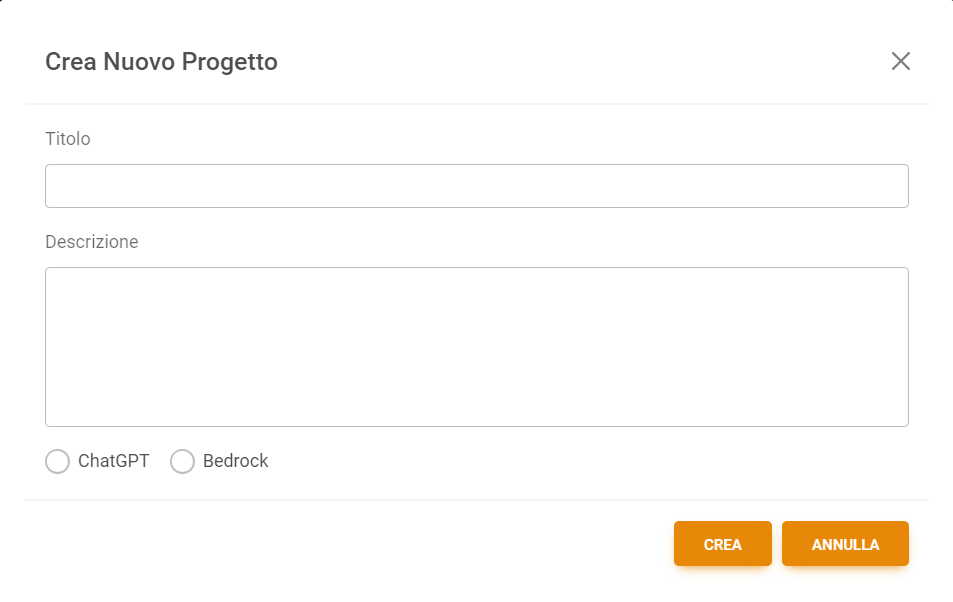
\includegraphics[width=\textwidth]{documenti/Screenshot manuale utente/crea nuovo progetto.png}
      \caption{Pagina delle notifiche}
      \label{notifiche}
    \end{figure} 
    Tramite il quale potrà creare un progetto
    \begin{itemize}
        \item Inserendo il titolo del progetto nel campo testuale "Titolo";
        \item Inserendo una descrizione testuale nel campo "Descrizione";
        \item Scegliendo l'intelligenza artificiale da utilizzare, cliccando sul pallino alla sinistra della scelta, che si evidenzierà e apparirà nel seguente modo:
        \begin{figure}[h]
      \centering
      
\includegraphics{documenti/Screenshot manuale utente/scelta ai.png}
      \caption{Scelta AI}
      \label{sceltaai}
    \end{figure} 
        \item Creare il progetto tramite il pulsante "Crea";
        \item Annullare l'operazione di creazione tramite il pulsante "Annulla".
    \end{itemize}
    \item Visualizzare la lista dei progetti
    \begin{figure}[H]
      \centering
      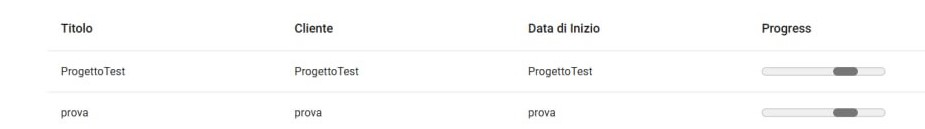
\includegraphics[width=\textwidth]{documenti/Screenshot manuale utente/lista prog def.jpeg}
      \caption{Lista dei progetti}
      \label{listaprog}
    \end{figure} 
    Le colonne della tabella dei progetti sono:
    \begin{itemize}
        \item Il Titolo, che indica il titolo attribuito al progetto;
        \item Il Cliente, dunque chi ha commissionato il progetto;
        \item La Data di inizio, che indica la data di creazione del progetto;
        \item La Progress bar, che mostra lo stato di avanzamento nello sviluppo del progetto.
    \end{itemize}
    Cliccando sulla freccetta che compare andando sopra il titolo di una colonna, è possibile invertire l'ordine alfabetico delle righe, A-Z oppure Z-A.
    \item Andare alla pagina successiva nel caso i progetti siano troppo numerosi per essere visualizzati all'interno della pagina. 
    \begin{figure}[H]
      \centering
      
\includegraphics[width=\textwidth]{documenti/Screenshot manuale utente/cambio pagina.png}
      \caption{Cambio pagina della lista}
      \label{paginalista}
    \end{figure} 
    A sinistra sono indicate le righe per pagina, modificabili tramite il menù a tendina visionabile cliccando sulla freccia a sinistra del numero delle righe e scegliendo il numero desiderato:
        \begin{figure}[H]
      \centering
      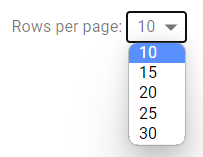
\includegraphics{documenti/Screenshot manuale utente/scelta righe per pagina.png}
      \caption{Scelta del numero di righe per pagina}
      \label{nrighepad}
    \end{figure} 
    è poi presente il numero della pagina in cui ci si trova rispetto al totale delle pagine, e le frecce per spostarsi all'interno di esse. Le frecce centrali permettono di spostarsi di una pagina rispettivamente precedente e successiva a quella in cui ci si trova, mentre le sue frecce esterne permettono di tornare rispettivamente alla prima o all'ultima pagina.
\end{itemize}

\subsubsection{Pagina delle Epic Stories}
Cliccando sulla riga del progetto di interesse (vedi immagine "Lista dei progetti"), è possibile vedere le Epic story del relative a quel progetto:
    \begin{figure}[H]
      \centering
      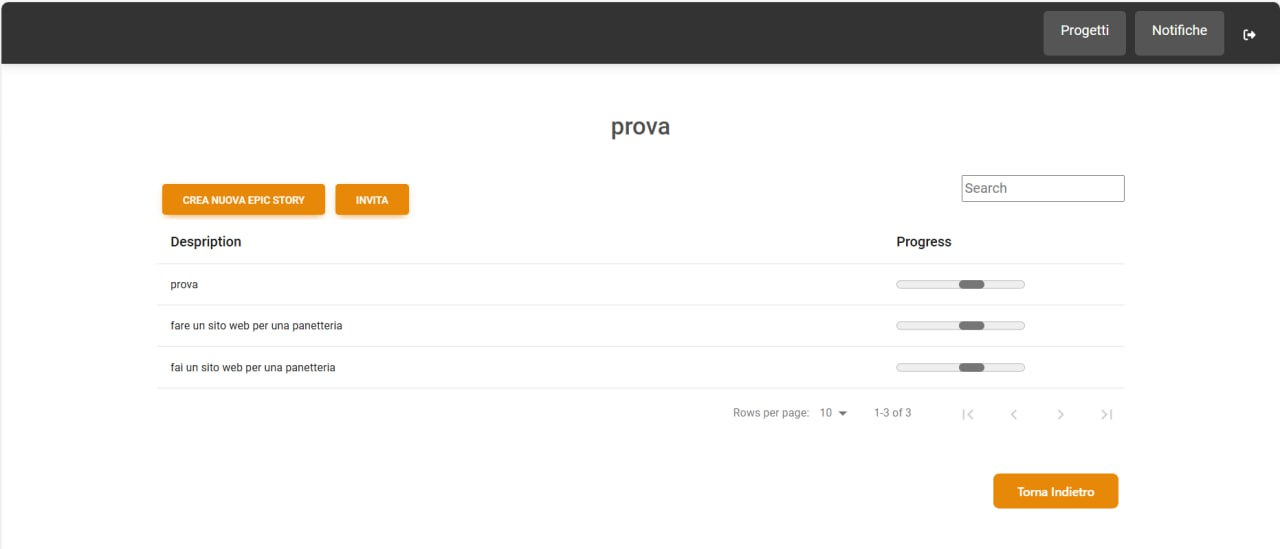
\includegraphics[width=\textwidth]{documenti/Screenshot manuale utente/epic pm.jpeg}
      \caption{Lista delle Epic stories}
      \label{listaepic}
    \end{figure} 
Le colonne della tabella indicano:
\begin{itemize}
    \item Il Nome delle Epic stories;
    \item La Descrizione delle Epic stories;
    \item Il Progress, ovvero una barra che indica lo stato di avanzamento delle Epic stories.
\end{itemize}
Cliccando sulla freccetta che compare andando sopra il titlolo di una colonna, è possibile invertire l'ordine alfabetico delle righe, A-Z oppure Z-A.\\\\

Cliccando sulla freccetta che compare andando sopra il titlolo di una colonna, è possibile invertire l'ordine alfabetico delle righe, A-Z oppure Z-A.\\\\
Tramite il pulsante in alto a sinistra "Crea nuova Epic story" è possibile creare una nuova Epic Story e apparirà il seguente pop-up:
    \begin{figure}[H]
      \centering
      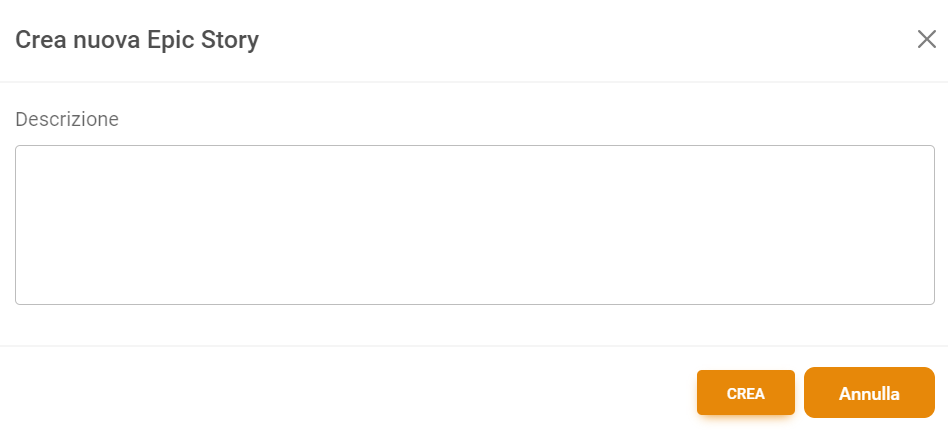
\includegraphics[width=\textwidth]{documenti/Screenshot manuale utente/creazione epic story.png}
      \caption{Creazione di un'Epic story}
      \label{creaepic}
    \end{figure} 
Per creare una nuova Epic story è necessario:
\begin{itemize}
    \item Inserire una descrizione testuale nel campo "Descrizione";
    \item Premere il pulsante "Crea" per creare l'invito;
    \item Se si desidera annullare l'operazione basterà cliccare il pulsante "Annulla".
\end{itemize}

Tramite il pulsante "Invita" a destra del pulsante "Crea nuova Epic story" è presente il pulsante "Invita", che permette di invitare degli utenti alla visualizzazione di un progetto, e dunque delle sue Epic e User story. Una volta cliccato apparirà il seguente pop-up:
    \begin{figure}[H]
      \centering
      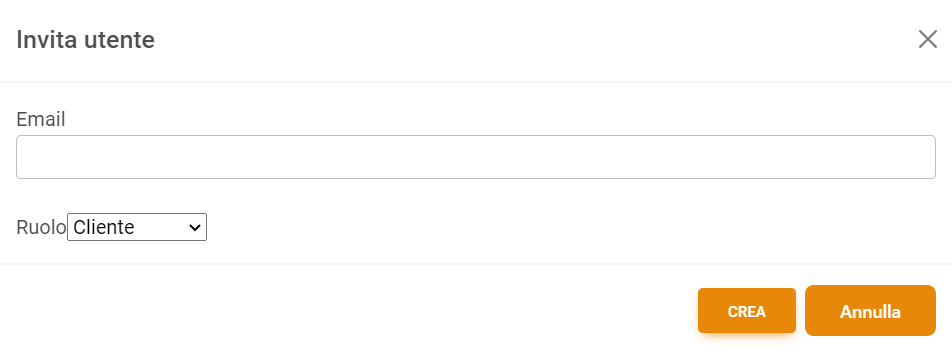
\includegraphics[width=\textwidth]{documenti/Screenshot manuale utente/invita utente.png}
      \caption{Invita un utente}
      \label{invitautente}
    \end{figure}
In cui è necessario: 
\begin{itemize}
    \item Inserire l'email di chi si desidera invitare;
    \item Scegliere il suo ruolo cliccando la freccia presente nel menù a tendina che apparirà nel seguente modo e selezionandolo:
        \begin{figure}[H]
      \centering
      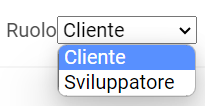
\includegraphics{documenti/Screenshot manuale utente/ruolo utente invitato.png}
      \caption{Scelta ruolo utente invitato}
      \label{ruolo invito}
    \end{figure}
    \item Cliccare il tasto "Crea" per finalizzare l'operazione;
    \item Se si desidera annullare l'operazione darà sufficiente cliccare il tasto "Annulla".
\end{itemize}

\subsubsection{Pagina delle User stories}
Cliccando sulla riga deell'Epic story di interesse (vedi immagine "Lista delle Epic stories"), è possibile vedere le User story del relative a quell'Epic story:
    \begin{figure}[H]
      \centering
      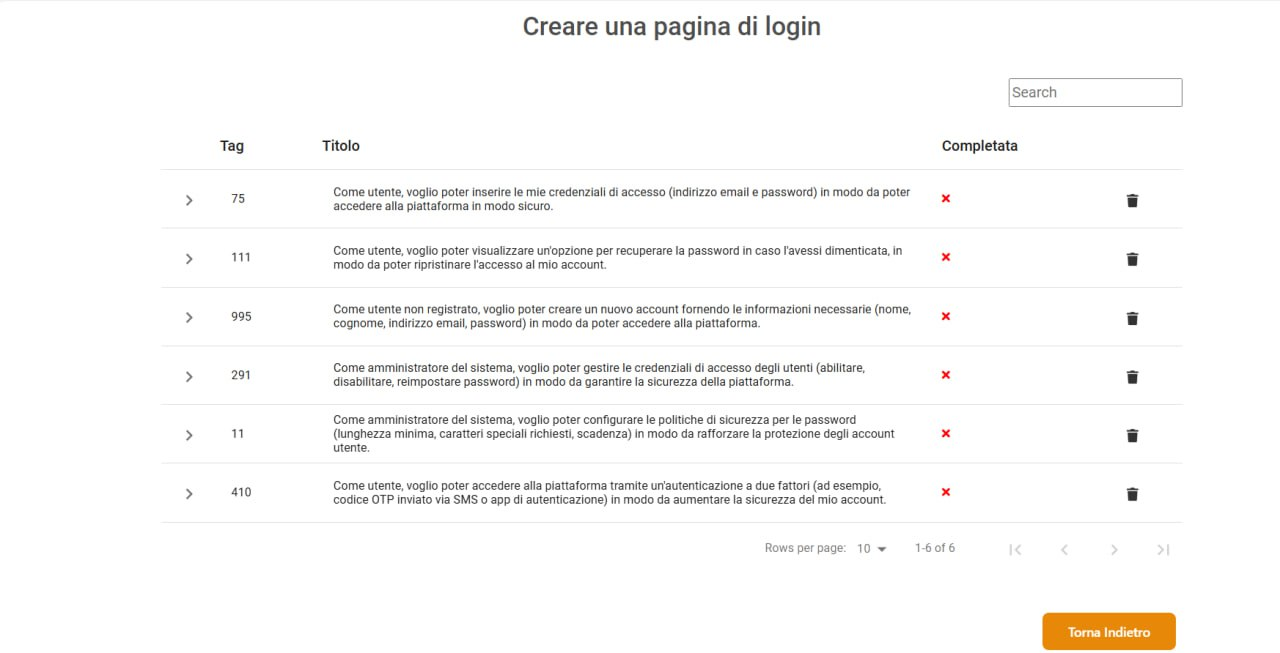
\includegraphics[width=\textwidth]{documenti/Screenshot manuale utente/us pm dev.jpeg}
      \caption{Lista delle User stories}
      \label{lista user}
    \end{figure}
Le colonne della tabella rappresentano: 
\begin{itemize}
    \item Il Tag, identificatore univoco delle User stories;
    \item Titolo delle User story;
    \item "Completata" che indica, nel caso di una croce rossa che non sia completata, nel caso di un tic verde che è stata completata.
\end{itemize}
A destra di ogni riga è presente l'icona di un cestino.
    \begin{figure}[H]
      \centering
      
\includegraphics{documenti/Screenshot manuale utente/cestino.png}
      \caption{Pulsante Elimina}
      \label{delete}
    \end{figure} 
    Cliccando il cestino sarà possibile eliminare una User. Per finalizzare l'operazione, una volta cliccata l'icona, apparirà la seguente schermata: 
        \begin{figure}[H]
      \centering
      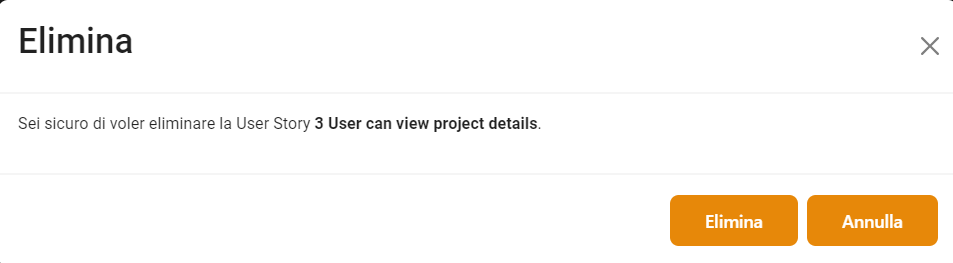
\includegraphics[width=\textwidth]{documenti/Screenshot manuale utente/delete us.png}
      \caption{Eliminazione User story}
      \label{deleteuser}
    \end{figure} 
    \begin{itemize}
        \item Per finalizzare l'eliminazione sarà sufficiente cliccare "Elimina";
        \item Se si desidera annullare l'operazione, basterà cliccare "Annulla".
        \item Le User story completate vengono eliminate all'interno della pagina ma restano presente nel database, in modo da permettere il conteggio personale delle ore impiegate nello sviluppo.
    \end{itemize}
Per visualizzare il dettaglio di una singola User story è sufficiente cliccare sulla riga della tabella corrispondente alla User story e la riga si espanderà verso il basso:
    \begin{figure}[H]
      \centering
      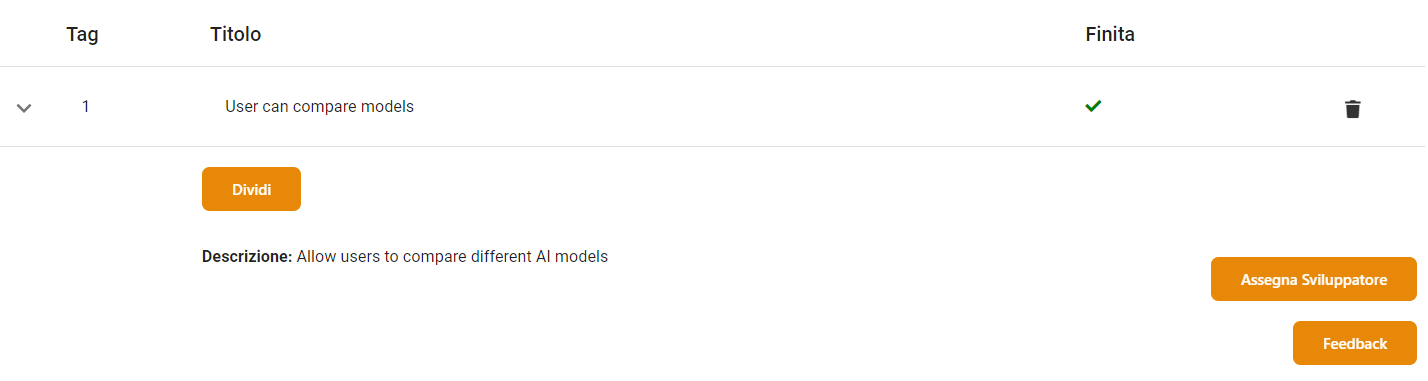
\includegraphics[width=\textwidth]{documenti/Screenshot manuale utente/dett us.png}
      \caption{Dettaglio delle User stories}
      \label{dettaglio user}
    \end{figure}
In questa sezione è possibile:
\begin{itemize}
    \item Cliccando sul pulsante "Dividi" è possibile inviare una richiesta all'intelligenza artificiale per dividere le User story in User story più piccole che ricaricando la pagina saranno visibili;
    \item Visionare la descrizione dell'User story;
    \item Assegnerà l'User story ad uno o più sviluppatori tramite il pulsante "Assegna sviluppatore". Cliccando sul pulsante apparirà il seguente pop-up:
        \begin{figure}[H]
      \centering
      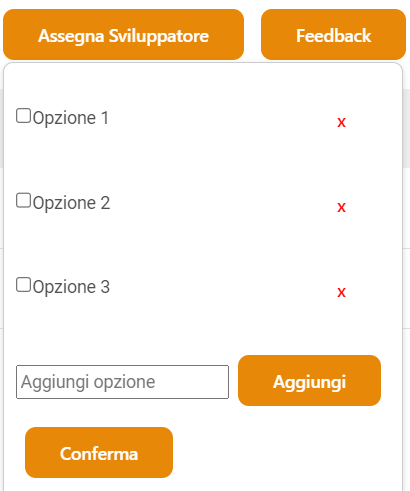
\includegraphics{documenti/Screenshot manuale utente/assegna sviluppatore.png}
      \caption{Assegnazione sviluppatori}
      \label{assegnadev}
    \end{figure}
    In questo pop-up per completare l'operazione di assegnazione è necessario:
    \begin{itemize}
        \item Cliccare il quadratino a sinistra della mail dello o degli sviluppatori ai quali si vuole assegnare, che si evidenzierà nel seguente modo: 
        \begin{figure}[H]
      \centering
      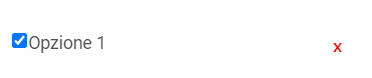
\includegraphics{documenti/Screenshot manuale utente/selezione sviluppatore.png}
      \caption{Selezione dello sviluppatore}
      \label{seldev}
    \end{figure}
    \item Se lo sviluppatore non è presente tra le opzioni, inserire la mail dello sviluppatore che si desidera nel campo testuale "Aggiungi opzione" e cliccare il pulsante "Aggiungi";
    \item Per completare l'operazione di assegnazione cliccare il pulsante "Conferma".
    \end{itemize}
    \item Aggiungere un feedback da inviare all'intelligenza artificiale. Cliccando il pulsante feedback apparirà il seguente pop-up:
    \begin{figure}[H]
      \centering
      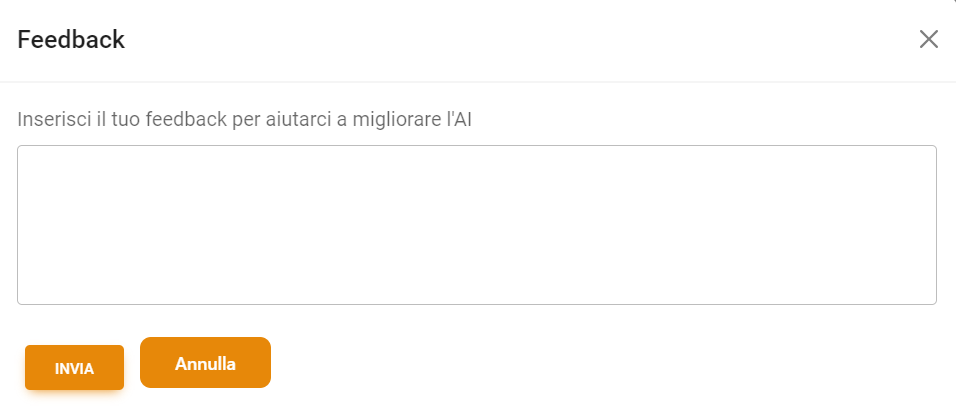
\includegraphics[width=\textwidth]{documenti/Screenshot manuale utente/feedback.png}
      \caption{Invio del feedback}
      \label{feedback}
    \end{figure}
    Per inviare un feedback è necessario:
    \begin{itemize}
        \item Scrivere il feedback nel campo testuale;
        \item Cliccare sul tasto "Invia" per finalizzare l'operazione;
        \item Per annullare l'operazione è sufficiente cliccare sul pulsante "Annulla".
    \end{itemize}
\end{itemize}


\section{Sviluppatore}
\subsection{Pagina dei progetti}
Questa è la pagina principale dello sviluppatore:
 \begin{figure}[H]
      \centering
      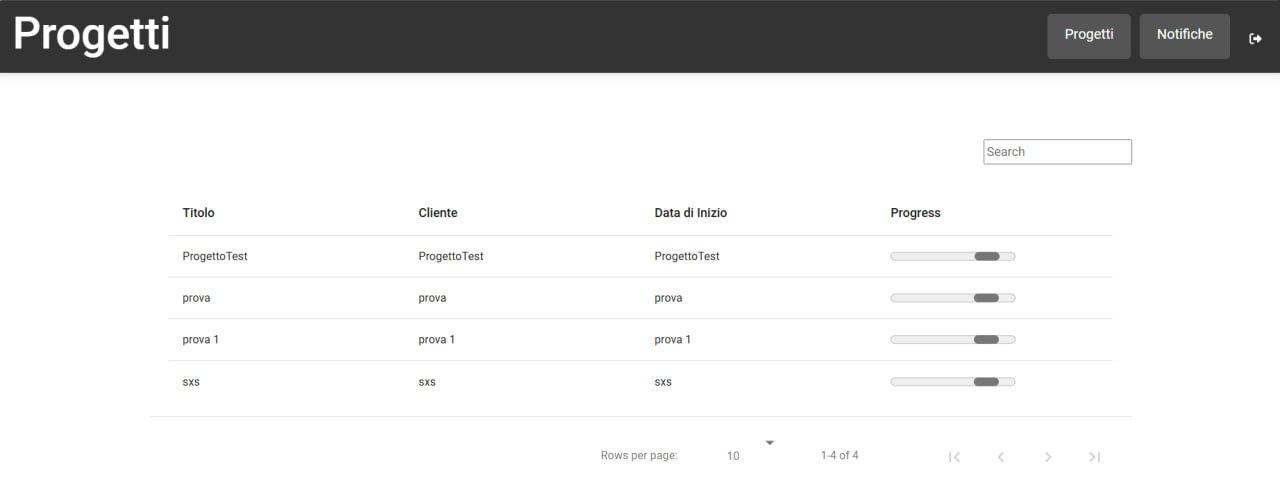
\includegraphics[width=\textwidth]{documenti/Screenshot manuale utente/home dev.jpeg}
      \caption{Pagina principale dello Sviluppatore}
      \label{pagdev}
    \end{figure} 
In questa pagina lo Sviluppatore può:
\begin{itemize}
    \item Visualizzare la lista dei progetti. Le colonne della tabella dei progetti sono:
    \begin{itemize}
        \item Il Titolo, che indica il titolo attribuito al progetto;
        \item Il Cliente, dunque chi ha commissionato il progetto;
        \item La Data di inizio, che indica la data di creazione del progetto;
        \item Il Progresso, cioè lo stato di avanzamento del progetto basato sulla percentuale di Epic e User stories completate.
    \end{itemize}
    Cliccando sulla freccetta che compare andando sopra il titolo di una colonna, è possibile invertire l'ordine alfabetico delle righe, A-Z oppure Z-A.
    \item Andare alla pagina successiva nel caso i progetti siano troppo numerosi per essere visualizzati all'interno della pagina. 
    \begin{figure}[H]
      \centering
      
\includegraphics[width=\textwidth]{documenti/Screenshot manuale utente/cambio pagina.png}
      \caption{Cambio pagina della lista}
      \label{paginalista}
    \end{figure} 
    A sinistra sono indicate le righe per pagina, modificabili tramite il menù a tendina visionabile cliccando sulla freccia a sinistra del numero delle righe e scegliendo il numero desiderato:
        \begin{figure}[H]
      \centering
      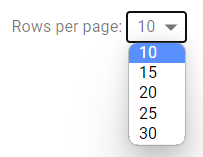
\includegraphics{documenti/Screenshot manuale utente/scelta righe per pagina.png}
      \caption{Scelta del numero di righe per pagina}
      \label{nrighepad}
    \end{figure} 
    è poi presente il numero della pagina in cui ci si trova rispetto al totale delle pagine, e le frecce per spostarsi all'interno di esse. Le frecce centrali permettono di spostarsi di una pagina rispettivamente precedente e successiva a quella in cui ci si trova, mentre le sue frecce esterne permettono di tornare rispettivamente alla prima o all'ultima pagina.
\end{itemize}

\subsubsection{Pagina delle Epic Stories}
Cliccando sulla riga del progetto di interesse (vedi immagine "Lista dei progetti), è possibile vedere le Epic story del relative a quel progetto:
    \begin{figure}[H]
      \centering
      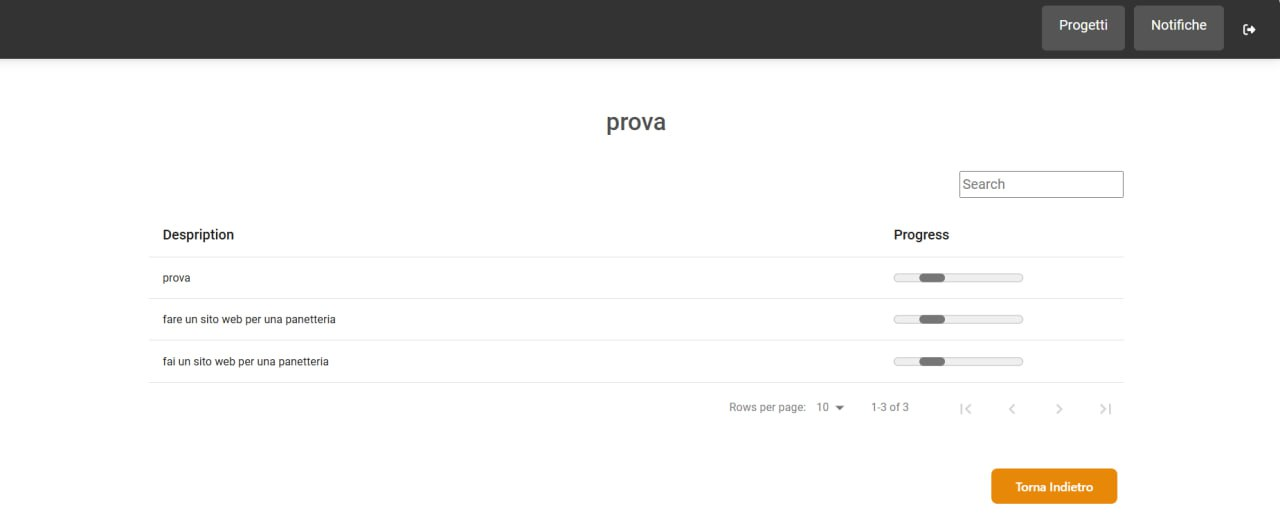
\includegraphics[width=\textwidth]{documenti/Screenshot manuale utente/epic dev.jpeg}
      \caption{Lista delle Epic stories}
      \label{listaepic}
    \end{figure} 
Le colonne della tabella indicano:
\begin{itemize}
    \item La Descrizione delle Epic stories;
    \item Il Progress, ovvero una barra che indica lo stato di avanzamento delle Epic stories.
\end{itemize}
Cliccando sulla freccetta che compare andando sopra il titlolo di una colonna, è possibile invertire l'ordine alfabetico delle righe, A-Z oppure Z-A.

\subsubsection{Pagina delle User stories}
Cliccando sulla riga deell'Epic story di interesse (vedi immagine "Lista delle Epic stories"), è possibile vedere le User story del relative a quell'Epic story:
    \begin{figure}[H]
      \centering
      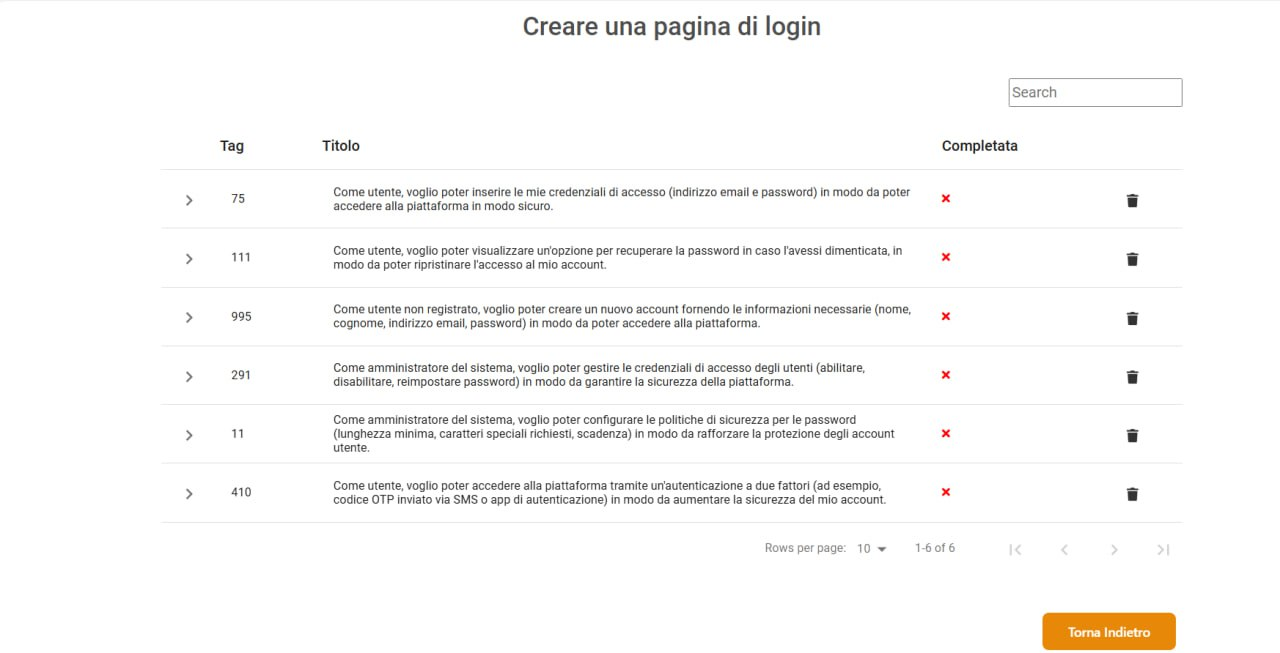
\includegraphics[width=\textwidth]{documenti/Screenshot manuale utente/us pm dev.jpeg}
      \caption{Lista delle User stories}
      \label{lista user}
    \end{figure}
Le colonne della tabella rappresentano: 
\begin{itemize}
    \item Il Tag, univoco per ogni User story;
    \item Titolo delle User story;
    \item "Completata" che indica, nel caso di una croce rossa che non sia completata, nel caso di un tic verde che è stata completata.
\end{itemize}
A destra di ogni riga è presente l'icona di un cestino.
    \begin{figure}[H]
      \centering
      
\includegraphics{documenti/Screenshot manuale utente/cestino.png}
      \caption{Pulsante Elimina}
      \label{delete}
    \end{figure} 
    Cliccando il cestino sarà possibile eliminare una User. Per finalizzare l'operazione, una volta cliccata l'icona, apparirà la seguente schermata: 
        \begin{figure}[H]
      \centering
      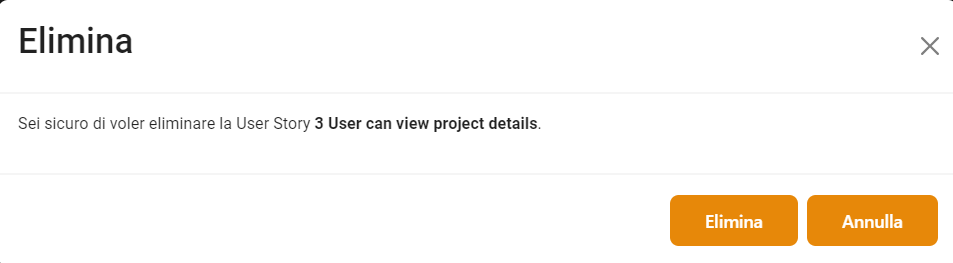
\includegraphics[width=\textwidth]{documenti/Screenshot manuale utente/delete us.png}
      \caption{Eliminazione User story}
      \label{deleteuser}
    \end{figure} 
    \begin{itemize}
        \item Per finalizzare l'eliminazione sarà sufficiente cliccare "Elimina";
        \item Se si desidera annullare l'operazione, basterà cliccare "Annulla".
        \item Le User story completate vengono eliminate all'interno della pagina ma restano presente nel database, in modo da permettere il conteggio personale delle ore impiegate nello sviluppo.
    \end{itemize}
Per visualizzare il dettaglio di una singola User story è sufficiente cliccare sulla riga della tabella corrispondente alla User story e la riga si espanderà verso il basso:
    \begin{figure}[H]
      \centering
      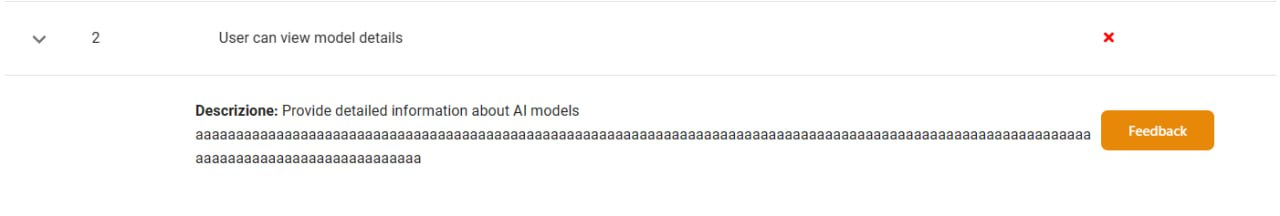
\includegraphics[width=\textwidth]{documenti/Screenshot manuale utente/dettaglio userstory dev.jpeg}
      \caption{Dettaglio delle User stories}
      \label{dettaglio user}
    \end{figure}
In questa sezione è possibile:
\begin{itemize}
    \item Visionare la descrizione dell'User story;
    \item Aggiungere un feedback da inviare all'intelligenza artificiale. Cliccando il pulsante feedback apparirà il seguente pop-up:
    \begin{figure}[H]
      \centering
      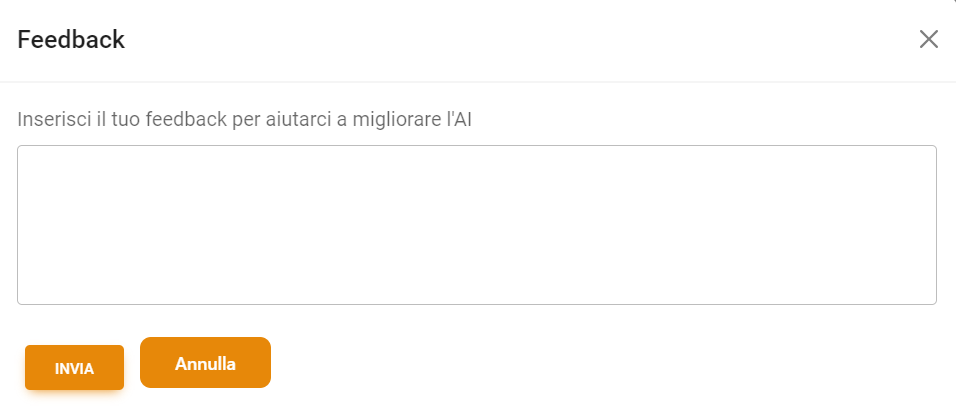
\includegraphics[width=\textwidth]{documenti/Screenshot manuale utente/feedback.png}
      \caption{Invio del feedback}
      \label{feedback}
    \end{figure}
    Per inviare un feedback è necessario:
    \begin{itemize}
        \item Scrivere il feedback nel campo testuale;
        \item Cliccare sul tasto "Invia" per finalizzare l'operazione;
        \item Per annullare l'operazione è sufficiente cliccare sul pulsante "Annulla".
    \end{itemize}
\end{itemize}

\section{Istruzioni per l'utilizzo del PlugIn}
\subsection{Introduzione}
Nella seguente sezione sono illustrate le funzionalità del PlugIn ed essendo destinato a sviluppatori, si presuppone un tipo di utilizzatore più esperto.

\subsection{Avvio del PlugIn}
\subsection{Istuzioni per l'utilizzo}
\subsubsection{Scelta della cartella e login}
Dopo aver aperto VSCode, all'avvio del PlugIn, apparirà automaticamente un pop-up per la scelta della cartella del progetto in cui si vuole lavorare:
    \begin{figure}[H]
      \centering
      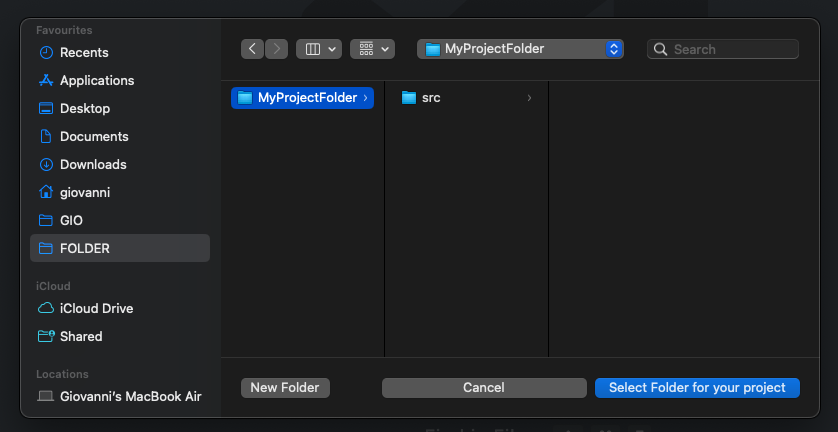
\includegraphics[width=\textwidth]{documenti/Screenshot manuale utente/folder-selection.png}
      \caption{Scelta della cartella di lavoro}
      \label{feedback}
    \end{figure}
    Per selezionare la cartella è necessario:
    \begin{itemize}
        \item Selezionare la cartella del progetto e cliccare "Select folder for your project";
        \item Se si desidera annullare l'operazione sarà sufficiente cliccare "Cancel".
    \end{itemize}
Una volta scelta la cartella di lavoro, a destra dell'editor di testo di testo di VSCode apparirà una colonna adibita alle funzionalità del PlugIn, con un login:
    \begin{figure}[H]
      \centering
      \includegraphics{documenti/Screenshot manuale utente/ban plugin.png}
      \caption{Login PlugIn}
      \label{loginplugin}
    \end{figure}
Per finalizzare l'operazione di login è necessario:
\begin{itemize}
    \item Inserire la propria email nel campo testuale "Email";
    \item Inserire la propria password nel campo testuale "Password";
    \item Cliccare il pulsante "Submit" per accedere.
\end{itemize}
Nel caso la email o la password inserite non siano corrette, apparirà il seguente messaggio di errore in basso a destra dello schermo:
    \begin{figure}[H]
      \centering
      \includegraphics{documenti/Screenshot manuale utente/errore login.png}
      \caption{Errore nel login PlugIn}
      \label{errlogplg}
    \end{figure}
    Nel caso si riscontrino problemi durante l'accesso provare a contattare il \hyperlink{linkSup}{supporto tecnico}. \\
Se lo username risulta inesistente contattare il \hyperlink{linkSup}{supporto tecnico}.
Una volta eseguito correttamente il login apparirà il seguente messaggio di conferma in basso a destra dello schermo: 
    \begin{figure}[H]
      \centering
      \includegraphics{documenti/Screenshot manuale utente/utente loggato.png}
      \caption{Utente loggato correttamente}
      \label{logcorretto}
    \end{figure}
    \subsubsection{Utilizzo delle funzionalità riguardanti le User story}
Simultaneamente alla comparsa del messaggio di login, nella sezione precedentemente occupata dal login apparirà la seguente schermata principale, contenente tutte le funzionalità del PlugIn:
    \begin{figure}[H]
      \centering
      \includegraphics[width=0.4\textwidth]{documenti/Screenshot manuale utente/vista_user_story.png}
      \caption{}
      \label{}
    \end{figure}
In questa schermata è possibile visualizzare tutte le User story assegnate. Cliccando sulla singola User story, si espanderà e sarà possibile visualizzarla nel dettaglio, con la sua associata descrizione.
    \begin{figure}[H]
      \centering
      \includegraphics[width=0.5\textwidth]{documenti/Screenshot manuale utente/dettaglio_user_story.png}
      \caption{Dettaglio della singola User story}
      \label{usdett}
    \end{figure}
Ogni User story, a sinistra del suo nome, è contrassegnata da una croce rossa o un tic verde, rispettivamente indicatori del fatto che la relativa user story abbia o meno passato tutti i suoi test.\\
\\
    \begin{figure}[H]
      \centering
      \includegraphics{documenti/Screenshot manuale utente/croce.png}
      \caption{Test dell'User story non superati}
      \label{testnonsup}
      \end{figure}
    \hfill
    \begin{figure}[H]
      \centering
      \includegraphics{documenti/Screenshot manuale utente/tic.png}
      \caption{Test dell'User story superati}
      \label{testsup}
    \end{figure}
\\

A sinistra del nome di ogni singola User Story, è presente un pulsante con un'icona di una pozione
    \begin{figure}[H]
      \centering
      \includegraphics{documenti/Screenshot manuale utente/pozione.png}
      \caption{Avvio dei test per la User story}
      \label{testus}
    \end{figure}
necessaria per avviare i test di quella User story. Per avviare i test è necessario:
\begin{itemize}
    \item Aprire il file relativo alla User story di interesse;
    Il file dovrà presentarsi rispettando la seguente struttura:
       \begin{figure}[H]
      \centering
      \includegraphics[width=\textwidth]{documenti/Screenshot manuale utente/example_file_with_tags.png}
      \caption{File di esempio}
      \label{exfile}
    \end{figure}
    \begin{itemize}
        \item Nella prima riga deve presentare la riga
        \begin{verbatim}
            //@PROJECT-tagprogetto 
        \end{verbatim} e sostituire "tagprogetto" con il reale tag del progetto.
        \item l'intero il codice della User story deve essere preceduto da 
        \begin{verbatim}
            //@USERSTORY-tagprogetto-taguserstory
        \end{verbatim} e sostituire "tagprogetto" con il reale tag del progetto, "taguserstory" con il reale tag della User story.
        \item alla fine del codice deve essere presente
        \begin{verbatim}
            //@USERSTORY-tagprogetto-taguserstory
        \end{verbatim}e sostituire "tagprogetto" con il reale tag del progetto, "taguserstory" con il reale tag della User story.
    \end{itemize}
    \item Cliccare l'icona della pozione.
\end{itemize}
Se non è mai stato generato un test relativo all'User story di interesse, il PlugIn crea una sottocartella a quella selezionata come cartella di lavoro, nomintata \textit{"TEST"} con al suo interno i file di test generati dall'AI, delle varie User story corrispondenti, nominati:
\begin{center}
    \begin{verbatim}
        UserStory_tagprogetto_taguserstory.test.ts 
    \end{verbatim} con al posto di "tagprogetto" il reale tag del progetto, "taguserstory" con il reale tag della User story.
\end{center}
Infine, cliccando l'icona della rotellina in alto a destra
    \begin{figure}[H]
      \centering
      \includegraphics{documenti/Screenshot manuale utente/rotellina.png}
      \caption{Avvio di tutti i test}
      \label{avvtest}
    \end{figure}
verranno runnati tutti i file all'interno della cartella "TEST" e il PlugIn agigornerà lo stato della User story controllando se tutti i test siano stati passati o meno, aggiornando il database e cambiando l'icona dello stato della User story.













\section{Supporto Tecnico}
\hypertarget{linkSup}{Per} eventuali malfunzionamenti durante l’utilizzo dell’applicazione, si prega di contattare il supporto tecnico inviando una email all’indirizzo:
\begin{center}
    \textbf{cybersorcerers23@gmail.com}
\end{center}
Si prega di utilizzare il seguente formato per la mail per evitare l'accidentale mancata visione delle richieste di supporto:
\begin{itemize}
    \item Oggetto: “nome dell’evento da segnalare”;
    \item Corpo;
    \item Data in cui si è riscontrato il malfunzionamento;
    \item Descrizione del malfunzionamento in esame;
    \item Sistema operativo e browser in cui si è verificato il problema;
    \item Allegato (facoltativo): immagini utili per la descrizione del malfunzionamento.
\end{itemize}


\end{document}
